\chapter{Synchronous Data Flow}\label{data-flow}\index{data flow!synchronous}

Engineers use difference equations for modelling discrete-time systems.
Computer science speaks of synchronous data flow models.  The
synchronous programming language \lustre~\cite{lustre} is based on this
model as is \signal~\cite{signal}.  The data flow sub language of \se\
borrows much of the syntax and semantics of \lustre.

\section{Discrete Data Flow}\label{data-flow-informal}

\paragraph{Difference equations.}\index{difference equation}
A low pass filter removes the higher frequencies in a signal while passing the lower frequencies. A simple low pass filter is, for instance, specified by a \emph{difference equation} such as
% 
$$y[n] = 0.1 * x[n] + 0.9 * y[n-1]$$
% 
The index abstracts time since $n$ really stands for $t = nT$ where $T$ is an interval of time. Thus the equation is a shorthand for 
% 
$$y[nT] = 0.1 * x[nT] + 0.9 * y[(n-1)T]$$
% 
which should be read as ``at time $nT$ the value of of $y$ is equal to the sum of the the value of $x$ at time $nT$ multiplied by $0.1$ and of the value of $y$ at time $(n-1)T$ multiplied by $0.9$''.
:
Synchronous programming speaks of data flow equations rather than of
difference equations. There is a shift in semantics as well:
$x$ and $y$ are considered just as sequences of data with the value of $y$ being determined from that of $x$ in discrete steps by applying the difference equation. No timing is involved. In particular, no assumptions are made that the intervals in between two steps will be of equal length.

Flow equations abstract from indexes. The $n-1$ is replaced by an
explicit operator (\texttt{pre} in \se)
%
\begin{center}
\pp{y := 0.1 * x -> 0.1 * x + 0.9 * pre(y); }
\end{center}
%
The operator \pp{pre(x)} refers to the status of the signal \pp{x} at the 
\emph{previous} index.\footnote{Some may be
reminded of the Z-tranform.} The operator \pp{->} (\emph{arrow}) 
distinguishes between the  \emph{first} index -- the 
value being determined by the initialisation \pp{a0 * x} --, and 
\emph{later} indexes -- the value being determined by 
the expression \pp{a0 * x + a1 * pre(x) + b1 * pre(y)}.

\paragraph{Traces.} We will define the semantics of flow equations 
in terms of traces. Traces have been used in Chapter~\ref{classes} to
illustrate reactive behaviour. We will now start to use traces as a basis
for the semantics of reactive behaviour.

Let a \emph{trace}\index{trace} be a sequence of data (of the same type). At an instant,
a trace may be \emph{accessible}\index{accessible} or \emph{inaccessible}\index{inaccessible}. If it is accessible it has a value. For visualisation, we use a diagram of the form
\begin{center}
  \leavevmode
  \begin{tabular}[]{l@{\quad}||@{\quad} cccccccc}
    \hline\hline   
     \hbox{{\footnotesize \textit{i}}} &{\footnotesize \textit{0}}
     &{\footnotesize \textit{1}}&{\footnotesize \textit{2}}
     &{\footnotesize \textit{3}}&{\footnotesize \textit{4}}
     &{\footnotesize \textit{5}}&{\footnotesize \textit{6}}&\ldots
   \\  
    \hbox{$d$} &&$d_0$&$d_{1}$&&&$d_2$&&\ldots
   \\
   \hline\hline
  \end{tabular}
\end{center}
The trace $d$ is accessible at an instant if there is an entry $d_{n}$. An empty slot marks inaccessibility. The index $i$ indicates the instants.


Standard operators lift to the corresponding traces by defining the operations
element-wise at every instant, e.g.
\begin{center}
  \leavevmode
  \begin{tabular}[]{l@{\quad}||@{\quad} cccccccc}
    \hline\hline
     \hbox{{\footnotesize \textit{i}}} &{\footnotesize \textit{0}}
     &{\footnotesize \textit{1}}&{\footnotesize \textit{2}}
     &{\footnotesize \textit{3}}&{\footnotesize \textit{4}}
     &{\footnotesize \textit{5}}&{\footnotesize \textit{6}}&\ldots
   \\  
    \hbox{$d$} &&$d_0$&$d_1$&&&$d_2$&&\ldots
   \\
    \hbox{$d'$} &&$d'_0$&$d'_1$&&&$d'_2$&&\ldots
   \\
    \hbox{$d + d'$} 
    &&$d_0+d'_0$&$d_1+d'_1$&&&$d_2+d'_2$&&\ldots
   \\ 
   \hline\hline
  \end{tabular}
\end{center}
The definition requires that $d$, $d'$, and $d + d'$ are accessible at the same instant. 

Literals and variables determine traces. For instance, the literal \pp{3} determines a trace that has the value $3$ at every instant
\begin{center}
  \leavevmode
  \begin{tabular}[]{l@{\quad}||@{\quad} cccccccc}
    \hline\hline
     \hbox{{\footnotesize \textit{i}}} &{\footnotesize \textit{0}}
     &{\footnotesize \textit{1}}&{\footnotesize \textit{2}}
     &{\footnotesize \textit{3}}&{\footnotesize \textit{4}}
     &{\footnotesize \textit{5}}&{\footnotesize \textit{6}}&\ldots
   \\  
     \hbox{$d$} &$3$&$3$&$3$&$3$&$3$&$3$&$3$&\ldots
   \\
   \hline\hline
  \end{tabular}
\end{center}


\paragraph{Shifting time.}\index{time shift}\index{pre@\pp{pre}}
The operator $pre(d)$ shifts the trace $d$ in that it pointwise refers
to the \emph{previous} element 
\begin{center}
  \leavevmode
  \begin{tabular}[]{l@{}||@{\quad} cccccccc}
    \hline\hline
     \hbox{{\footnotesize \textit{i}}} &{\footnotesize \textit{0}}
     &{\footnotesize \textit{1}}&{\footnotesize \textit{2}}
     &{\footnotesize \textit{3}}&{\footnotesize \textit{4}}
     &{\footnotesize \textit{5}}&{\footnotesize \textit{6}}&\ldots
   \\  

    \hbox{$d$ \quad} &&$d_0$&$d_1$&&&$d_2$&&\ldots
   \\
    \hbox{\texttt{pre($d$)} \quad}  
    &&$\delta$&$d_0$&&&$d_1$&&\ldots
   \\
   \hline\hline
  \end{tabular}
\end{center}
The first element is a default value since there is no previous element. $\delta$ is a (type dependent, e.g. $0$ for integers, $false$ 
for booleans) default value. The trace \pp{pre($d$)} is accessible if and only if $d$ is accessible.

\paragraph{Initialising a trace.}\index{arrow (\pp{->})} The arrow operator distinguishes between the very first element of a trace, and all later elements.  
\begin{center}
  \leavevmode
  \begin{tabular}[]{l@{\quad}||@{\quad} cccccccc}
    \hline\hline
     \hbox{{\footnotesize \textit{i}}} &{\footnotesize \textit{0}}
     &{\footnotesize \textit{1}}&{\footnotesize \textit{2}}
     &{\footnotesize \textit{3}}&{\footnotesize \textit{4}}
     &{\footnotesize \textit{5}}&{\footnotesize \textit{6}}&\ldots
   \\  
    \hbox{$d$ \quad} &&$d_0$&$d_1$&&&$d_2$&&\ldots
   \\
    \hbox{$d'$} &&$d'_0$&$d'_1$&&&$d'_2$&&\ldots
   \\
   \hbox{\texttt{$d$ -> $d'$} } &&$d_0$&$d'_1$&&&$d'_2$&&\ldots
   \\
   \hline\hline
  \end{tabular}
\end{center}
The first element of the trace \texttt{$d$ -> $d'$} is the first element $d_{0}$ of the trace $d$ while the other elements are those of the trace $d'$. Note again that all the traces should be accessible at the same 
instants.

\paragraph{Flow equations.}\index{flow!equation}
The traces corresponding to a flow equation are inductively defined 
folllowing the structure of flow expressions. Here are two examples. The 
first example is an incrementing counter defined by the data flow 
equation
%
$$\pp{count := 0 -> pre(count) + 1;}$$
%
Here \texttt{count} is a signal of type \texttt{int}. At an instant,
the signal may be constrained by the flow equation, i.e. its value
is updated to be equal to the value of the expression on the right hand side. 
Hence the following behaviour is enforced.
\begin{center}
  \leavevmode
  \begin{tabular}[]{l@{\quad}||@{\quad}ccccccccccc}
    \hline\hline   
     \hbox{{\footnotesize \textit{i}}} &{\footnotesize \textit{0}}
     &{\footnotesize \textit{1}}&{\footnotesize \textit{2}}
     &{\footnotesize \textit{3}}&{\footnotesize \textit{4}}
     &{\footnotesize \textit{5}}&{\footnotesize \textit{6}}&\ldots
   \\  
    \hbox{$count$} 
    &$\mathbf{0}$&$\mathbf{1}$&$\textbf{2}$&$\mathbf{3}$&$\mathbf{4}$&
    $\mathbf{5}$&$\mathbf{6}$&$\mathbf{7}$&\ldots
   \\
    \hbox{$pre(count)$} &$\mathbf{0}$&$\mathit{0}$&$\mathit{1}$&$\mathit{2}$&
    $\mathit{3}$&$\mathit{4}$&$\mathit{5}$&$\mathit{6}$&\ldots
   \\    
    \hbox{$pre(count) + 1$} 
    &$\mathit{1}$&$\mathit{1}$&$\mathit{2}$&$\mathit{3}$&
    $\mathit{4}$&$\mathit{5}$&$\mathit{6}$&$\mathit{7}$&\ldots
   \\
    \hbox{$0\ \pp{->}\ pre(count) + 1$} 
	 &$\mathit{0}$&$\mathit{1}$&$\mathit{2}$&$\mathit{3}$&
	 $\mathit{4}$&$\mathit{5}$&$\mathit{6}$&$\mathit{7}$&\ldots
   \\
     \hline\hline
  \end{tabular}
\end{center} 
%For $n = 0$, we have $x(0) = 0$ due to the arrow operator. By 
%induction we can then prove that $x(n) = n$ for all $n$.
Let us assume that the signal \texttt{count} is updated at every instant
(implying that the signal is accessible). Let us say that a signal is present
if it is constrained by a flow equation. Presence is indicated by the bold typeface. 

In case of the (Boolean) flow expression 
%
$$\pp{raising\_edge : = false -> x \&\& !pre(x)}$$
%
 we may have the following table ($f$ stands for \emph{false}, and 
$t$ for \emph{true}) 
\begin{center}
  \leavevmode
  \begin{tabular}[]{l@{}||@{\quad}ccccccccccc}
    \hline\hline
     \hbox{{\footnotesize \textit{i}}} &{\footnotesize \textit{0}}
     &{\footnotesize \textit{1}}&{\footnotesize \textit{2}}
     &{\footnotesize \textit{3}}&{\footnotesize \textit{4}}
     &{\footnotesize \textit{5}}&{\footnotesize \textit{6}}
     &{\footnotesize \textit{7}}&\ldots
   \\  
    \hbox{$x$}
    &$f$&$t$&$t$&$f$&$f$&$t$&$f$&$t$&\ldots
   \\ 
    \hbox{$pre(x)$} &$f$&$f$&$t$&$t$&$f$&$f$&$t$&$f$&\ldots
   \\    
    \hbox{$! pre(x)$} &$t$&$t$&$f$&$f$&$t$&$t$&$f$&$t$&\ldots
   \\
    \hbox{$x\ {\tiny \&\&}\ !\ pre(x)$} &$f$&$t$&$f$&$f$&$f$&$t$&$f$&$t$&\ldots
   \\
    \hbox{$false\ \pp{->}\ x\ {\tiny \&\&}\ !pre(x)$\quad}
		&$f$&$t$&$f$&$f$&$f$&$t$&$f$&$t$&\ldots
   \\
    \hbox{$raising\_edge$\quad}
		&$\mathbf{f}$&$\mathbf{t}$&$\mathbf{f}$&$\mathbf{f}$&
		$\mathbf{f}$&$\mathbf{t}$&$\mathbf{f}$&$\mathbf{t}$&\ldots
	\\   \hline\hline
  \end{tabular}
\end{center}
The expression detects what hardware people call a \emph{raising 
edge}, i.e. the instants when the signal \texttt{x} changes from \emph{false} 
to \emph{true}.

\paragraph{A uniform view of updating.}
We note that signals my be updated
\begin{itemize}
\item either by emitting it as explained in the previous chapter,

\item or by constraining it by a flow equation.
\end{itemize}
Though conceptually quite different, both methods of updating behave equivalently in that
\begin{itemize}
\item if a signal is updated, either by emitting or constraining, it is present with a new value (if valued), and in that

\item multiple updating, either by emitting or constraining, of a signal at 
the same instant is a time race causing an error message.
\end{itemize}
However,
\begin{itemize}
\item \emph{flow equations support a richer language} including the time 
shift operators (and sampling operations, as we will learn in Section~\ref{multi-clock}).
\end{itemize}
%


\section{Embedding Data Flow to Control}\label{embedding}

\paragraph{Flow contexts.}\index{flow!context|textbf}
Flow equations are only allowed to occur in a particular context of the form
$$\texttt{\{| \ldots\  |\}}$$
We speak of a \emph{flow context}. Its body consists of a sequence of
flow equations (and of local signal declarations, see below).

Restricting the occurrence of flow equations to a particular context has the advantage that ambiguity of typing can be avoided: we stipulate that 
\emph{only flows can occur within a flow context}.
 Then an expression such as \pp{3 + 5} 
then has different interpretations within or outside of a flow context.
\begin{itemize}
\item Outside of a flow context, the terms \pp{3}, \pp{5}, and \pp{3 + 5} denote integers, and the addition operation operates on integers.

\item Within a flow context, the terms \pp{3}, \pp{5}, and \pp{3 + 5} are integer flows, and the addition operator operates on integer flows.

\item \emph{Note the operators \pp{pre} and \pp{->} can only be used within a flow context.}
\end{itemize}

The order of presentation of flow equations within a flow context is 
irrelevant for evaluation. The flow equation are evaluated by an
order imposed by the equations: if a signal is used 
within a flow expression on some right its value must be computed 
before the expression can be evaluated (\emph{write-before-read}), except
if the signal is ``guarded'' by a \texttt{pre}. In that case, a value is used
that has been computed at some previous instant. Here are some schematic 
examples for illustration:
\begin{itemize}
\item The two flow contexts
%
\BEP
   \{|  x := 0 -> pre(y);
       y := 2 * x;
   |\}    
\EEP
%
and
%
\BEP
   \{|  y := 2 * x;
       x := 0 -> pre(y);
   |\} 
\EEP   
%
behave equivalently; the flow equation for signal \texttt{x} must be
evaluated before that for signal \texttt{y} since it is used on the right
hand side of the flow equation for signal \texttt{y}.

\item The flow equations 
%
\BEP
   \{|  x := 0 -> y;
       y := 2 * x;
   |\}    
\EEP
%
will raise a causality error\index{causality!cycle}. We have a cyclic dependency since the flow
equation for \texttt{x} uses the value of \texttt{y} of the same instant,
and vice versa. Note that guarding \texttt{y} with a \texttt{pre} in the
equations above breaks the cycle, since the value of \texttt{y} of a previous
instant is used.

\end{itemize}
The notation $\texttt{\{| \ldots\  |\}}$ is meant to indicate that the 
order of presentation of flow equations is not relevant. 
Of course, for each signal, there should be at most one flow equation in any
flow context.

\paragraph{The watchdog example.} We rephrase the ``watchdog'' example of \cite{halbwachs}. The watchdog is a device to manage deadlines. There are three Boolean signals \pp{set}, \pp{reset}, and \pp{deadline}. The signals
\pp{set} and \pp{reset} switch the watchdog ``on'' and ``off''. If the watchdog is ``on'', and if the signal \pp{deadline} is true, the signal \pp{alarm} is true.
%
\codefragment{watchdog-body}
%
The formulation uses the conditional.
A hardware designer might prefer to use Boolean operators only, which 
yields a (disputably) more elegant solution.
%
\codefragment{watchdog-bool}
%
Note that ``setting the watchdog'' has precedence over resetting. The
precedence is reversed by using
%
\codefragment{watchdog-bool-2}
%

\paragraph{Modes.}\index{mode} 
It is somewhat inherent that the  evaluation of flow equations 
should be sustained for some time. 
This is achieved by using (a variant of) the \pp{sustain}\index{sustain@\pp{sustain}} statement
%
\BEP
    sustain \{|
       \ldots
    |\};
\EEP
%
Once started, the \pp{sustain} process never terminates; flow 
constraints are applied forever. We shall speak of a \emph{mode} (of 
operation). The idea is that modes persist, usually for a long interval,
but modes may be changed if necessary, for instance from a start-up mode
to a working mode, or from a working mode to an error mode or maintenance mode, 
and vice versa.

Being a process like any other, the sustain statement may be preempted and (re-) started as in
%
\codefragment{counting-up}
%
A trace of this fragment may look like as follows
\begin{center}
  \leavevmode
  \begin{tabular}[]{l@{\quad}||@{\quad}ccccccccccccc}
    \hline\hline
     \hbox{{\footnotesize \textit{i}}} &{\footnotesize \textit{0}}
     &{\footnotesize \textit{1}}&{\footnotesize \textit{2}}
     &{\footnotesize \textit{3}}&{\footnotesize \textit{4}}
     &{\footnotesize \textit{5}}&{\footnotesize \textit{6}}
     &{\footnotesize \textit{7}}&{\footnotesize \textit{8}}
     &{\footnotesize \textit{9}}&\ldots
   \\      
   \hbox{$start$} &.&.&.&*&.&.&.&.&.&.&\ldots
   \\
    \hbox{$stop$} &.&.&.&.&.&.&*&.&.&.&\ldots
   \\     
   \hbox{$count$}&$\mathit{0}$&$\mathit{0}$&$\mathit{0}$&
   $\mathbf{1}$&$\mathbf{2}$&$\mathbf{3}$&
   $\mathbf{4}$&$\mathbf{5}$&$\mathit{4}$&$\mathit{4}$&\ldots
%   \\ 
%    \hbox{$pre(count)$} &.&.&.&$0$&$0$&$1$&$2$&$3$&$4$&.&\ldots
%   \\    
%    \hbox{$pre(count) + 1$} &.&.&.&$1$&$1$&$2$&$3$&$4$&$5$&.&\ldots
%   \\    
%    \hbox{$0\ \texttt{->}\ pre(count) + 1$}
%           &.&.&.&$0$&$1$&$2$&$3$&$4$&$5$&.&\ldots
   \\
  
  \hline\hline
  \end{tabular}
\end{center}
If the signal \texttt{start} is present, the flow context starts to be
sustained.  The flow equation is evaluated at every instant till
the signal \texttt{stop} is present. Whenever the flow equation is evaluated
the signal \texttt{count} is updated, hence increased. Then the sustained process terminates instantaneously when the signal \texttt{stop} is present. 

The presence of the pure signals \texttt{start} and
\texttt{stop} is indicated by an asterisk. The signal \texttt{start} is present at the 4th instant,
and the flow context is active from the 4th to the 8th instant.  

\paragraph{\textit{Mode automata.}}\label{mode-automata}\index{mode automaton} 
{\em If we combine state machines with flow equations we may consider states as corresponding to modes. This is the idea of \emph{mode automata} as 
presented in ~\cite{Maranchini}. The following example has two moses/states, counting upward and counting downward.
% 
\codeinput{up-and-down-counter-automaton}
%

The construction is somewhat clumsy in that we have to use the 
\pp{next} to avoid multiple constraints: since preemption is weak, 
the program may count upward, change state from \pp{\em up} to 
\pp{\em down}, and count downward at the same instant if the \pp{\em 
next} would not guard the \pp{\em sustain} clause. The idea, in fact, 
would be that the flow equations should be active only if a state is 
in control but not if control enters a state. Since this phenomenon 
is quite usual for mode automata, we allow to use flow equations in the 
\pp{\em during} clause of a state as in 
% 
\codeinput{up-and-down-counter-during}
%
Then the flow equations are active when being in a state,
 but not if entering a state. Thus multiple constraints are avoided.
}

\section{Flow Contexts and Locality}

\paragraph{Local Signals.}\index{signal!local}
Signals can be declared within a flow context as local variables. All the rules for local variables apply (cf. Section~\ref{local-signals}) except for
exception: the initialisation
may be dropped, i.e. the shorthand \texttt{Signal<$T$>} may be used instead of \texttt{Signal<$T$> = new Signal<$T$>();}.
The scope of the signal are all the subsequent statements within the flow context.

Of course, using local variables may substantially change behaviour. We
reconsider
%
\codefragment{counting-up-2}
%
If the \pp{sustain} statement is active, the signal \pp{count} is increased,
otherwise its value persists. A typical trace is
\begin{center}
  \leavevmode
  \begin{tabular}[]{l@{\quad}||@{\quad}ccccccccccccc}
    \hline\hline
     \hbox{{\footnotesize \textit{i}}} &{\footnotesize \textit{0}}
     &{\footnotesize \textit{1}}&{\footnotesize \textit{2}}
     &{\footnotesize \textit{3}}&{\footnotesize \textit{4}}
     &{\footnotesize \textit{5}}&{\footnotesize \textit{6}}
     &{\footnotesize \textit{7}}&{\footnotesize \textit{8}}
     &{\footnotesize \textit{9}}&\ldots
   \\      
    \hbox{$start$} &.&$*$&.&.&.&.&$*$&.&.&.&\ldots
   \\
    \hbox{$stop$} &.&.&.&$*$&.&.&.&$*$&.&.&\ldots
   \\     
   \hbox{$count$} &$\mathit{0}$&$\mathbf{1}$&$\mathbf{2}$&
   $\mathbf{3}$&$\mathit{3}$&$\mathit{3}$&
   $\mathbf{4}$&$\mathbf{5}$&$\mathit{5}$&$\mathit{5}$&\ldots
   \\ 
  \hline\hline
  \end{tabular}
\end{center}

If the signal \pp{count} is declared locally within the flow context, a new
incarnation of \pp{count} is generated when control enters the flow context.
%
\codefragment{counting-up-3}
%
The corresponding trace is 
\begin{center}
  \leavevmode
  \begin{tabular}[]{l@{\quad}||@{\quad}ccccccccccccc}
    \hline\hline
     \hbox{{\footnotesize \textit{i}}} &{\footnotesize \textit{0}}
     &{\footnotesize \textit{1}}&{\footnotesize \textit{2}}
     &{\footnotesize \textit{3}}&{\footnotesize \textit{4}}
     &{\footnotesize \textit{5}}&{\footnotesize \textit{6}}
     &{\footnotesize \textit{7}}&{\footnotesize \textit{8}}
     &{\footnotesize \textit{9}}&\ldots
   \\      
    \hbox{$start$} &.&$*$&.&.&.&.&$*$&.&.&.&\ldots
   \\
    \hbox{$stop$} &.&.&.&$*$&.&.&.&$*$&.&.&\ldots
   \\          
   \hbox{$count'$} &&$\mathbf{1}$&$\mathbf{2}$&$\mathbf{3}$&&&&&&&\ldots
   \\
   \hbox{$pre(count')$} &&$\mathit{0}$&$\mathit{1}$&$\mathit{2}$&&&&&&&\ldots
   \\   
   \hbox{$pre(count')+1$}   &&$\mathit{1}$&$\mathit{2}$&
   $\mathit{3}$&&&&&&&\ldots
   \\
   \hbox{$count''$} &&&&&&&$\mathbf{1}$&$\mathbf{2}$&&&\ldots
   \\  
   \hbox{$pre(count'')$} &&&&&&&$\mathit{0}$&$\mathit{1}$&&&\ldots
   \\  
   \hbox{$pre(count'')+1$} &&&&&&&$\mathit{1}$&$\mathit{2}$&&&\ldots
   \\
  \hline\hline
  \end{tabular}
\end{center}
Why is this so? Whenever
the flow context is started, a new incarnation of the signal \pp{count} is created. Since this incarnation is clearly not accessible at previous instants, \pp{pre(count)} is initialised with 
a default value (here $0$). 

\paragraph{The \texttt{pre} operator and locality.}\index{pre@\pp{pre}!locality of} The operator \pp{pre} may
be applied to an expression as in
%
\codeinput{counting-up-4}
%
We consider the expression \pp{pre(count + 1)} as a shorthand for
%
\codeinput{counting-up-5}
%
with the local signal name \pp{aux} being chosen appropriately. 
This implies that the value of the expression is set to a default value when
starting the flow context. The corresponding traces look like this
\begin{center}
  \leavevmode
  \begin{tabular}[]{l@{\quad}||@{\quad}ccccccccccccc}
    \hline\hline
     \hbox{{\footnotesize \textit{i}}} &{\footnotesize \textit{0}}
     &{\footnotesize \textit{1}}&{\footnotesize \textit{2}}
     &{\footnotesize \textit{3}}&{\footnotesize \textit{4}}
     &{\footnotesize \textit{5}}&{\footnotesize \textit{6}}
     &{\footnotesize \textit{7}}&{\footnotesize \textit{8}}
     &{\footnotesize \textit{9}}&\ldots
   \\      
    \hbox{$start$} &.&$*$&.&.&.&.&$*$&.&.&.&\ldots
   \\
    \hbox{$stop$} &.&.&.&$*$&.&.&.&$*$&.&.&\ldots
   \\          
   \hbox{$count$} &$\mathit{0}$&$\mathbf{0}$&$\mathbf{1}$&$\mathbf{2}$
   &$\mathit{2}$&$\mathit{2}$&$\mathbf{0}$&$\mathbf{1}$&
   $\mathit{1}$&$\mathit{1}$&\ldots
   \\
   \hbox{$count + 1$} &&$\mathit{1}$&$\mathit{2}$&$\mathit{3}$&
   &&$\mathit{1}$&$\mathit{2}$&&&\ldots
   \\   
   \hbox{$pre(count + 1)$} &&$\mathit{0}$&$\mathit{1}$&
   $\mathit{2}$&&&$\mathit{0}$&$\mathit{1}$&&&\ldots
   \\     \hline\hline
  \end{tabular}
\end{center}
The result may be \emph{surprising}. The general idea is that expressions within a flow context are accessible only if the flow context is active. Otherwise the expressions -- hence the result of is evaluation -- is inaccessible.

Since this may be confusing we issue a general warning:
\begin{itemize}
\item \emph{\textbf{All usages of the operator \emph{\pp{pre}} should be properly guarded by an initialisation using the arrow operator.}}
\end{itemize}


\paragraph{The arrow operator and locality.}\index{arrow (\pp{->})!locality of}

Initialisation by an arrow operator takes place \emph{whenever a flow context is started}. Consider
%
\codeinput{counting-up-6} with the signal \pp{count} being globally defined.
Whenever \pp{start} is present the flow context is started, and the signal count is initialised to $0$.
\begin{center}
  \leavevmode
  \begin{tabular}[]{l@{\quad}||@{\quad}ccccccccccccc}
    \hline\hline
     \hbox{{\footnotesize \textit{i}}} &{\footnotesize \textit{0}}
     &{\footnotesize \textit{1}}&{\footnotesize \textit{2}}
     &{\footnotesize \textit{3}}&{\footnotesize \textit{4}}
     &{\footnotesize \textit{5}}&{\footnotesize \textit{6}}
     &{\footnotesize \textit{7}}&{\footnotesize \textit{8}}
     &{\footnotesize \textit{9}}&\ldots
   \\      
    \hbox{$start$} &.&$*$&.&.&.&.&$*$&.&.&.&\ldots
   \\
    \hbox{$stop$} &.&.&.&$*$&.&.&.&$*$&.&.&\ldots
   \\          
   \hbox{$count$} &$\mathit{0}$&$\mathbf{0}$&$\mathbf{1}$&$\mathbf{2}$
   &$\mathit{2}$&$\mathit{2}$&$\mathbf{0}$&$\mathbf{1}$&
   $\mathit{1}$&$\mathit{1}$&\ldots
   \\     \hline\hline
  \end{tabular}
\end{center}
Remember that without initialisation the counter is increased steadily 
whenever the flow context is active.

\noindent\emph{Remark.} One may be seduced by as expression such as
%
\BEP
  x := 0 -> (1 -> pre(x) + 1 )
\EEP
%
to believe that the value of \pp{x} is $0$ at the first instant when starting a flow context, and $1$ at the second. However, the definition says that,
whatever the trace on the right hand side of \pp{0 -> \ldots} is, the value
is $0$ at the first instant. Hence the flow equation above behaves equivalently to
%
\BEP
  x := 0 -> pre(x) + 1
\EEP
%

\paragraph{\textit{Hybrid systems.}}\index{system!hybrid}\label{hybrid-system}
\emph{We use ``localised'' versions of the pre and the arrow operator to support
the specification of hybrid systems. Hybrid systems are characterized by the interaction of continuous parts, governed by differential or difference equations (difference equations only in our context), and by discrete parts, described by finite state machines, if-then-else rules, propositional and temporal logic. Hybrid systems switch between many operating modes where each mode is governed by its own characteristic dynamical laws. Mode transitions are triggered by variables crossing specific thresholds (state events), by the elapse of certain time periods (time events), or by external inputs (input events). Further it is usually required that each mode starts operating with defined initial conditions specified by a reset relation.
}

\emph{In \se, all ``continuous'' modes are encapsulated by flow context, while all
the other language constructs specify the discrete parts resp. the transitions. Now having local initialisation by the arrow operators provides
the means to specify a reset relation. The initial condition can depend 
on the status of (globally declared) signals at a previous instant that is accessed by using the operator \pp{pre}. This is the sort of rationale for
our ``localised'' interpretation of the operators \pp{->} and \pp{pre}.}\footnote{Note that this generalises the use of these operators in \lustre. \lustre\ programs have -- in our terminology -- only one mode. Hence initialisation by the arrow operator can take place only in the very first instant, as well as the operator \pp{pre} has a default value only in the first instant (forgetting about 
, see Section~\ref{multi-clock}).}


\emph{To give a simple example of a typical presentation of a hybrid systems we consider a bouncing ball with the following properties:}
\begin{itemize}
\item \emph{Motion is characterised by \emph{height} ($x_{1}$) and \emph{vertical} velocity ($x_{2}$)},
\item \emph{Continuous changes between bounces.}
\item \emph{Discrete change at bounce time.}
\item \emph{Dynamics summarised by}
\begin{itemize}
\item \emph{one \emph{mode} $q$ with a continuous behaviour specified by the equations}
\begin{eqnarray*}
\dot{x_{1}} & = & x_{2}\\
\dot{x_{2}} & = & -g
\end{eqnarray*}
 
\item \emph{one \emph{transition} from $q$ to $q$ guarded by the condition $h \leq 0$,
}\item \emph{a reset relation that keeps the height but reverses the direction of velocity and decreases it by a factor in that $x_{2}$ is set to 
$-cx_{2}$.} 
\end{itemize}
\end{itemize}

\emph{The behaviour is graphically specified by}
\begin{center}
	{\tt\small
       \thinlines
       \setlength{\unitlength}{0.9pt}
       \begin{picture}(140,100)
           \put(5,70){$x_{1} \leq 0$}
           \put(90,70){$x_{2} := -cx_{2}$}
           \put(65,76){\circle{50}}
           \put(79,59){\thicklines\vector(-2,-1){7}}
          \put(30,0){\Ovalbox{\begin{Beqnarray*}
                                      \\\ \dot{x_{1}} & = & x_{2}\
                                      \\\dot{x_{2}} & = & -g\\
                                 \end{Beqnarray*}}}       
       \end{picture}
     }
\end{center}
\emph{If we try to translate this to a program, the obvious is to 
replace an differential equation $\dot{x} = e$ is replaced by an integral 
$x = x_{0} +\int edx$, and to compute the integral using difference
equations such as, for instance:}
\begin{itemize}
  \item \emph{(forward) Euler}
	\begin{eqnarray*}
		  x_{1}(n) & = & x_{1}(n-1) + x_{2}(n-1) \times dt \\
		  x_{2}(n) & = & \left\{
		                  \begin{array}{lll}
		                       -c*x_{2}(n-1) &- g*dt&\mbox{if $x_{1} \le 0$} \\
		                          x_{2}(n-1) &- g*dt&\mbox{otherwise}
		                    \end{array}
		               \right.
	\end{eqnarray*}
  \item \emph{or backward Euler}
	\begin{eqnarray*}
		  x_{1}(n) & = & x_{1}(n-1) + x_{2}(n) \times dt \\
		  x_{2}(n) & = & \left\{
		                  \begin{array}{lll}
		                       -c*x_{2}(n-1) &- g*dt&\mbox{if $x_{1} \le 0$} \\
		                          x_{2}(n-1) &- g*dt&\mbox{otherwise}
		                    \end{array}
		               \right.
	\end{eqnarray*}
\end{itemize}	
\emph{Another choice maybe Runge-Kutta. For the example, backward Euler works. A corresponding \se\ program is}
%
\codeinput{bouncing-ball}
%
\emph{Whenever the state \pp{move} is entered, the speed is reversed. Note that 
forward Euler would fail: whenever the direction switches, the speed
is negative before the switch, and positive after. For backward Euler, we
would compute \emph{\pp{x1 := pre(x1) + pre(x2) * dt}} after the switch, but with
\pp{pre(x2)} which is the negative value of speed before the switch. Hence,
the height would decrease rather than increase after the switch, actully be 
less than $0$ again, causing another switch. Hence the height toggles about
$0$ while the speed decreases, which does not quite reflect the physics. }

\paragraph{\textit{Warning}} \emph{If compared with simulation tools such as
 Matlab/Simulink or Scilab/Scicos one should note that in case of 
 ``zero-crossings'' resolution of computation cannot be improved for
 better results: the $dt$ provides the finest resolution.
One should keep here in mind that the language is build for hard real-time
control. Hence we cannot artificially ``stretch time'' as can
be achieved for offline simulators. 
}

\emph{Hence one should not use an exact value such as $0.0$ for changing direction
but rather some $\epsilon$ ball, meaning replacing $o.o$ by a small positive value.}

\section{Examples}

\subsection{Using Flows for the Stopwatch}\label{stopwatch-flow}

 
\paragraph{The simple stopwatch.} The following fragment rephrases the
simple stopwatch of Section~\ref{stopwatch} using flow equations
%
\codeinput{flow-simple-stopwatch}
%
The signal \pp{running} is toggled if the sensor \pp{start\_stop} is true.
The displayed time is increased if in the running state, reset to $0$ if
the sensor \pp{reset} is true, and otherwise kept unchanged. 

\paragraph{The general stopwatch.}
The general stopwatch permits to record intermediate times. As in Section~\ref{stopwatch}, we introduce a signal \pp{elapsed\_time} that behaves like the signal \pp{display\_time} of the simple stopwatch. For the general stopwatch the signal \pp{display\_time} remains constant if the stopwatch is in state ``frozen''.  The signal
\pp{reset} has two functionalities: (i) if the stopwatch is stopped but not frozen then the time is reset to $0$ (by the signal \pp{actual\_reset}, and (b) it toggles between the states ``frozen'' and ``not froozen''.
%
\codeinput{flow-simple-stopwatch-with-intermediate-time}
%

\paragraph{\textit{The general stopwatch as a hybrid system.}}
\emph{The logic of the general stopwatch is quite intriguing and needs careful analysis for a proper understanding. This is due to the fact that the effect of sporadic control features such as pushing the \emph{\pp{start\_stop}} button or 
the \emph{\pp{reset}} button are implemented using logic. Using hybrid systems provides a much clearer design
%
\codeinput{flow-hybrid-stopwatch}
%
In state \emph{\pp{running}} both the internal and the displayed times are increased. In state \emph{\pp{frozen}} only the internal time is increased. One realizes that the stopwatch can be reset to \emph{\pp{0sec}} only if the process is neither in state \emph{\pp{running}} nor in state \emph{\pp{frozen}}. Further if being stopped the \emph{\pp{start\_stop}} button has precedence over the \emph{\pp{reset}} button. In the pure flow version this is rather implicit in that for evaluating the flow equation for the internal time the \emph{\pp{actual\_reset}} condition is only checked if the system is not running.}

\subsection{The Train Example Reconsidered.}\label{train-flow}
We rephrase the single line train example \ref{train} using data 
flow. We replace all the input and output signals by Boolean signals.  
There are two additional Boolean signals \pp{change} and 
\pp{priority}. The signal \pp{change} computes any change 
situation, and signal \pp{priority} the priority of trains 
as the name suggests. The priority is computed only if a change of 
situation takes place in that a new train arrives or a train leaves 
the single track.
To compute the change and the priority there are three more auxiliary 
Boolean signals \pp{trainWaiting}, 
\pp{trainArriving}, and \pp{lineFreed}. The latter is true at the 
instant a train leaves the single line. The meaning of the other two 
are obvious. 
% 
\codefragment{train-data-flow-equations}
%
The overall behaviour should be easy to grasp considering the 
explanations
given in Section~\ref{train}. The pointings are set according to the 
priority, and the traffic lights are set to green when the obvious 
conditions hold.

\subsection{The LEGO Example using Flows}

We present a flow variant of the robot example in
Section~\ref{lego-example}.  The wheeled robot is able to move
forward and backward, and to turn left and right.  Two bumper sensors
on the left and right front end are used to detect obstacles.  The
task is to control the robot such that it travels around without
being caught, for instance, in some corner.

\codeinput{travel-flow}

The sensors are encoded by the sensors \pp{lsensor}
and \pp{rsensor}. The motor actuators are \pp{ldir}, \pp{rdir}, 
\pp{lspeed}, and \pp{rspeed}.

\section{Reusing Data Flow Equations}

\paragraph{Block diagrams.}\index{block diagram} Engineers often prefer a visual 
presentation for data flows, e.g.
\begin{center}
	{\tt\small
       \thinlines
       \setlength{\unitlength}{0.9pt}
       \begin{picture}(220,50)
           \put(5,15){x}

           \put(0,25){\vector(1,0){120}}

           \put(20,5){\vector(1,0){10}}

           \put(20,25){\line(0,-1){20}}
           \put(30,0){\framebox(30,10){\footnotesize pre}}       
           \put(60,5){\vector(1,0){20}}

           \put(80,0){\framebox(20,10){!}}       
           \put(100,5){\line(1,0){10}}
           \put(110,5){\line(0,1){10}}
           \put(110,15){\vector(1,0){10}}

           \put(120,10){\framebox(20,20){\&\&}}       
           \put(140,20){\vector(1,0){50}}

           \put(145,15){
               \begin{picture}(60,35)
                   \put(0,25){\framebox(40,10){\footnotesize false}}
                   \put(15,15){\line(0,1){10}}
                   \put(15,15){\vector(1,0){25}}
                   \put(40,0){\framebox(20,20){->}}
               \end{picture}
           }
       \put(210,25){\vector(1,0){30}}

       \put(227,15){y}

       \end{picture}
     }
 \end{center}
The boxes represent operators (with constants being an operator of 
arity 0),  and arrows represent flows of data between these. The 
behaviour corresponds to that of the flow equation for finding a
raising edge
%
\BEP
y := false.. -> x \&\& ! pre(x);
\EEP
% 
Typically such block diagrams are abstracted by boxing in the diagram as in    
\begin{center}
 {\tt\small
   \thinlines
   \setlength{\unitlength}{0.8pt}
   \begin{picture}(120,25)
       \put(10,14){$x$}
       \put(90,14){$y$}
       \put(0,10){\vector(1,0){30}}
       \put(80,10){\vector(1,0){30}}          
       \put(30,0){\framebox(50,20){edge\_up}} 
             \end{picture}
 }
\end{center}
The new box may be used in other diagrams as a shorthand as in 
the following fragment of the train example in Section~\ref{train}
\begin{center}
 {\tt\scriptsize
   \thinlines
   \setlength{\unitlength}{0.8pt}
   \begin{picture}(440,100)
       \put(405,48){change}
       \put(400,45){\vector(1,0){40}}
       \put(380,30){\framebox(20,30){||}} 
       \put(370,55){\vector(1,0){10}}
       \put(370,55){\line(0,1){20}}
       \put(360,75){\line(1,0){10}}
 	    \put(340,60){\framebox(20,25){\&\&}} 
       \put(320,65){\vector(1,0){20}}
       \put(260,85){trainArriving}
       \put(140,85){trainWaiting}
       \put(130,80){\vector(1,0){80}}
       \put(110,65){\framebox(20,30){||}} 
       \put(0,90){\vector(1,0){110}}
       \put(0,80){rightTrainWaiting}
       \put(0,70){\vector(1,0){110}}
       \put(0,60){leftTrainWaiting}
       \put(255,80){\vector(1,0){85}}
       \put(210,70){\framebox(45,20){edge\_up}} 
       \put(320,50){\line(0,1){15}}
       \put(0,50){\line(1,0){320}}
       \put(0,40){isLineFree}
       \put(70,5){\line(0,1){45}}
       \put(70,5){\vector(1,0){20}}
       \put(135,5){\vector(1,0){205}}          
       \put(140,8){lineFreed}
       \put(90,-5){\framebox(45,20){edge\_up}} 
       \put(170,25){\line(0,1){55}}
       \put(170,25){\vector(1,0){170}}
       \put(370,35){\vector(1,0){10}}
       \put(370,15){\line(0,1){20}}
       \put(360,15){\line(1,0){10}}
       \put(340,0){\framebox(20,30){\&\&}} 
   \end{picture}
 }
\end{center}

Block diagrams provide a natural abstraction mechanism for structuring and for reuse in the world of data flow corresponding to method calls in an object-oriented world.

\paragraph{A textual presentation.}  Looking for a textual representation of block diagrams, we observe that
\begin{itemize}
\item a block is specified in terms of
   \begin{itemize}
      \item ingoing and outgoing flows, and
      \item a body being a flow context and that 
    \end{itemize}

\item a block is embedded in a diagram by connecting  the flows inside and outside of the block. 
\end{itemize}

The mechanism we use resembles that of reactive methods, but the body
only consist of a flow context, e.g\index{edge\_up@\pp{edge\_up}}
%
\codefragment{edge-up}
%
We speak of \emph{nodes}\index{node|textbf} rather than of blocks, hence the keyword. For connection, sensors and signals are passed as parameters as in
%
\BEP
edge\_up(isLineFree,LineFreed)
\EEP
%
Calling the node within a flow context then ``glues'' the boxes.
\codefragment{data-flow-train-nodes}

When compiling, each node call\index{node!call} is expanded by replacing the parameters by the arguments and by adding its flow equations to the enclosing flow context.
In case of the train example the code to execute is
\codefragment{data-flow-train-nodes-expanded}

\paragraph{Relational abstraction.}\index{abstraction!relational}
The general scheme is to have boxes with $m$ ingoing flows and $n$ outgoing flows
\begin{center}
 {\tt\small
   \thinlines
   \setlength{\unitlength}{0.8pt}
   \begin{picture}(120,55)
       \put(10,44){$x_{1}$}
       \put(120,44){$y_{1}$}
       \put(0,40){\vector(1,0){30}}
       \put(110,40){\vector(1,0){30}} 
       \put(10,31){.}      
       \put(10,27){.}      
       \put(10,23){.}      
       \put(120,31){.}      
       \put(120,27){.}      
       \put(120,23){.}   
       \put(10,14){$x_{m}$}
       \put(120,14){$y_{n}$}
       \put(0,10){\vector(1,0){30}}
       \put(110,10){\vector(1,0){30}}          
       \put(30,0){\framebox(80,50){xxxx}} 
   \end{picture}
 }
\end{center}
The corresponding textual counterpart adds type information 
%
\BEP
node xxxx ( Sensor<$T_{1}$>$   x_{1}$, \ldots , Sensor<$T_{m}$>$   x_{m}$,
            Signal<$T_{m+1}$>$ y_{1}$, \ldots , Signal<$T_{m+n}$>$ y_{n}$ ) \{|

  ...
  
|\};
\EEP
%
The body is restricted to be a flow context.

A node specifies a relation for constraining flows, just as flow equations do. Hence a node may be only called within a flow context. If the flow context is active at an instant, the constraints of the flow equations apply as well as those that are specified by a node called.\footnote{Here, \se\ substantially differs from \lustre\ that uses functional abstraction.}

%We restrict the \emph{actual parameters of flow equations to be flow variables or flow signals only} for pragmatic reasons: if a parameter is ``outgoing'', i.e. it appears on the left side of a flow equation in the body of a flow method, then it should be constrained by the respective flow equation in that it the right hand side constrains the left hand side. This implicit direction of constraining flows would be violated if a flow expression such as, e.g. $3$, is an actual argument for an ``outgoing'' flow
%parameter. Though not strictly necessary, we apply the same convention for ``ingoing'' parameters. Though this may sometimes raise the need of adding auxiliary variables, the code tends to be more readable.

\paragraph{The stopwatch again.}
The stopwatch of Section~\ref{stopwatch-flow} is an example for using a flow method with multiple input and output flows. The simple stopwatch becomes the flow method
%
\codefragment{flow-stopwatch-method-simple-stopwatch}
%
This method is called within a flow context as follows
%
\codeinput{flow-stopwatch-general}
%

%\subsection{Functional Abstraction}\index{abstraction!functional}
%The example above might



\section{\textit{On Clocks}}\label{multi-clock}

{\em

\paragraph{\textit{Sampling signals.}}\index{sampling} 
Execution of a flow equations consumes real time. Hence one may sometimes 
want to avoid executing a data flow equation at every instant. Let, for 
example, the input $x$ of the filter equation 
$$y(n) = a_0 * x(n) + a_1 * x(n-1) - b_1 * y(n-1),$$
be given by a curve such as 
\begin{center}
 {\tt\scriptsize
   \thinlines
   \setlength{\unitlength}{1pt}
   \begin{picture}(205,60)
   \put(0,20){\line(1,0){205}}
   \put(5,30){\bezier{200}(0,20)(35,30)(55,-10)}
   \put(60,20){\bezier{200}(0,0)(15,-30)(30,0)}
   \put(90,20){\bezier{200}(0,0)(20,40)(70,20)}
   \put(160,20){\bezier{200}(0,20)(20,10)(40,20)}
   \put(5,20){\line(0,1){30}}   
   \put(10,20){\line(0,1){31}}   
   \put(15,20){\line(0,1){32}}   
   \put(20,20){\line(0,1){32}}   
   \put(25,20){\line(0,1){31}}   
   \put(30,20){\line(0,1){30}}   
   \put(35,20){\line(0,1){28}}   
   \put(40,20){\line(0,1){26}}   
   \put(45,20){\line(0,1){22}}   
   \put(50,20){\line(0,1){15}}   
   \put(55,20){\line(0,1){8}}
   \put(65,20){\line(0,-1){8}}   
   \put(70,20){\line(0,-1){13}} 
   \put(75,20){\line(0,-1){15}} 
   \put(80,20){\line(0,-1){13}} 
   \put(85,20){\line(0,-1){9}} 
   \put(95,20){\line(0,1){9}} 
   \put(100,20){\line(0,1){15}}
   \put(105,20){\line(0,1){19}} 
   \put(110,20){\line(0,1){22}}
   \put(115,20){\line(0,1){24}}
   \put(120,20){\line(0,1){25}}
   \put(125,20){\line(0,1){26}}
   \put(130,20){\line(0,1){26}}
   \put(135,20){\line(0,1){26}}
   \put(140,20){\line(0,1){25}}
   \put(145,20){\line(0,1){24}}
   \put(150,20){\line(0,1){23}}
   \put(155,20){\line(0,1){22}}
   \put(160,20){\line(0,1){20}}
   \put(165,20){\line(0,1){18}}
   \put(170,20){\line(0,1){17}}
   \put(175,20){\line(0,1){16}}
   \put(180,20){\line(0,1){15}}
   \put(185,20){\line(0,1){16}}
   \put(190,20){\line(0,1){17}}
   \put(195,20){\line(0,1){18}}
   \put(200,20){\line(0,1){20}}   
   \end{picture}
 }
\end{center}
For reasons of efficiency, one want to compute the filter equation only every other instant
\begin{center}
 {\tt\scriptsize
   \thinlines
   \setlength{\unitlength}{1pt}
   \begin{picture}(205,60)
   \put(0,20){\line(1,0){205}}
   \put(5,30){\bezier{200}(0,20)(35,30)(55,-10)}
   \put(60,20){\bezier{200}(0,0)(15,-30)(30,0)}
   \put(90,20){\bezier{200}(0,0)(20,40)(70,20)}
   \put(160,20){\bezier{200}(0,20)(20,10)(40,20)}
   \put(5,20){\line(0,1){30}}   
   \put(15,20){\line(0,1){32}}   
   \put(25,20){\line(0,1){31}}   
   \put(35,20){\line(0,1){28}}   
   \put(45,20){\line(0,1){22}}   
   \put(55,20){\line(0,1){8}}
   \put(65,20){\line(0,-1){8}}   
   \put(75,20){\line(0,-1){15}} 
   \put(85,20){\line(0,-1){9}} 
   \put(95,20){\line(0,1){9}} 
   \put(105,20){\line(0,1){19}} 
   \put(115,20){\line(0,1){24}}
   \put(125,20){\line(0,1){26}}
   \put(135,20){\line(0,1){26}}
   \put(145,20){\line(0,1){24}}
   \put(155,20){\line(0,1){22}}
   \put(165,20){\line(0,1){18}}
   \put(175,20){\line(0,1){16}}
   \put(185,20){\line(0,1){16}}
   \put(195,20){\line(0,1){18}}
   \end{picture}
 }
\end{center}
The filter equation turns into
$$y(2*n) = a_0 * x(2*n) + a_1 * x(2*(n-1)) - b_1 * y(2*(n-1))$$
The formalisation gets messy though if we want to sample the curve
only if its amplitude is below a certain threshold as in
\begin{center}
 {\tt\scriptsize
   \thinlines
   \setlength{\unitlength}{1pt}
   \begin{picture}(205,60)
   \put(0,20){\line(1,0){205}}
   \put(5,30){\bezier{200}(0,20)(35,30)(55,-10)}
   \put(60,20){\bezier{200}(0,0)(15,-30)(30,0)}
   \put(90,20){\bezier{200}(0,0)(20,40)(70,20)}
   \put(160,20){\bezier{200}(0,20)(20,10)(40,20)}
   \dashline{5}(0,42)(200,42)
   \put(45,20){\line(0,1){22}}   
   \put(50,20){\line(0,1){15}}   
   \put(55,20){\line(0,1){8}}
   \put(65,20){\line(0,-1){8}}   
   \put(70,20){\line(0,-1){13}} 
   \put(75,20){\line(0,-1){15}} 
   \put(80,20){\line(0,-1){13}} 
   \put(85,20){\line(0,-1){9}} 
   \put(95,20){\line(0,1){9}} 
   \put(100,20){\line(0,1){15}}
   \put(105,20){\line(0,1){19}} 
   \put(110,20){\line(0,1){22}}
   \put(155,20){\line(0,1){22}}
   \put(160,20){\line(0,1){20}}
   \put(165,20){\line(0,1){18}}
   \put(170,20){\line(0,1){17}}
   \put(175,20){\line(0,1){16}}
   \put(180,20){\line(0,1){15}}
   \put(185,20){\line(0,1){16}}
   \put(190,20){\line(0,1){17}}
   \put(195,20){\line(0,1){18}}
   \put(200,20){\line(0,1){20}}   
   \end{picture}
 }
\end{center}

\se\ provides a very simple mechanism to deal with down-sampling. The 
operator 
\begin{center}
\emph{\pp{$E$ when $C$}}
\end{center}
states that the expression $E$ is evaluated only if the condition $C$ 
becomes true. 

Hence the flow equations
\begin{quote}
\emph{\pp{y := (a0 * x + a1 * pre(x) + 
b1 * pre(y)) when c;\\
c := false -> !pre(c);}}
\end{quote}
express precisely that the filter equation is evaluated only every other
instant. Restricting sampling by a threshold is neatly expressed by 
\begin{quote}
\emph{\pp{y := (a0 * x + a1 * pre(x) + 
b1 * pre(y)) when (x < up);}}
\end{quote}
and both may be combined to
\begin{quote}
\emph{\pp{y := (a0 * x + a1 * pre(x) + 
b1 * pre(y)) when (c \& x < up);\\
c := false -> !pre(c);}}
\end{quote}
as visualised by
\begin{center}
 {\tt\scriptsize
   \thinlines
   \setlength{\unitlength}{1pt}
   \begin{picture}(205,60)
   \put(0,20){\line(1,0){205}}
   \put(5,30){\bezier{200}(0,20)(35,30)(55,-10)}
   \put(60,20){\bezier{200}(0,0)(15,-30)(30,0)}
   \put(90,20){\bezier{200}(0,0)(20,40)(70,20)}
   \put(160,20){\bezier{200}(0,20)(20,10)(40,20)}
   \dashline{5}(0,42)(200,42)
   \put(45,20){\line(0,1){22}}   
   \put(55,20){\line(0,1){8}}
   \put(65,20){\line(0,-1){8}}   
   \put(75,20){\line(0,-1){15}} 
   \put(85,20){\line(0,-1){9}} 
   \put(95,20){\line(0,1){9}} 
   \put(105,20){\line(0,1){19}} 
   \put(155,20){\line(0,1){22}}
   \put(165,20){\line(0,1){18}}
   \put(175,20){\line(0,1){16}}
   \put(185,20){\line(0,1){16}}
   \put(195,20){\line(0,1){18}}
   \end{picture}
 }
\end{center}

We used a bit of hand waving here. Precisely, the right hand side of the
equation is down-sampled only using the operator \emph{\pp{when}}, but not
the left hand side. If we reconsider the down-sampled filter equation
$$y(2*n) = a_0 * x(2*n) + a_1 * x(2*(n-1)) - b_1 * y(2*(n-1))$$
the down-sampling (multiplying by $2$) applies to both sides. We express
down-sampling of signals as an annotation to the signal type, e.g.
\begin{center}
\emph{\pp{Signal\{c \& x < up\}<double> y;}}
\end{center} 
We refer to the expression \emph{\emph{\pp{c \& x < up}}} as a \emph{clock}\index{clock}.
The idea is that a signal can only be updated by a flow constraint
at an instant if the clock condition evaluates to true at that instant.
Clearly, the signal and the expression on the right hand side of a flow
equation should ``be on the same clock'' (this will be made precise further below).

\paragraph{\textit{Sampling operators.}} 
The operator \emph{\pp{when}} \emph{down-samples}\index{down-sampling}\index{when@\pp{when}} the trace $d$ at a \emph{frequency} specified by the Boolean ``clock'' flow $c$ as in, e.g.,
\begin{center}
  \leavevmode
  \begin{tabular}[]{l@{\quad}||@{\quad} ccccccccccc}
    \hline\hline  
     \hbox{{\footnotesize \textit{i}}} &{\footnotesize \textit{0}}
     &{\footnotesize \textit{1}}&{\footnotesize \textit{2}}
     &{\footnotesize \textit{3}}&{\footnotesize \textit{4}}
     &{\footnotesize \textit{5}}&{\footnotesize \textit{6}}
     &{\footnotesize \textit{7}}&{\footnotesize \textit{8}}
     &{\footnotesize \textit{9}}&\ldots
   \\      
    \hbox{$d$} &&$d_0$&$d_{1}$&&&$d_2$&&$d_3$&$d_4$&&\ldots
   \\
    \hbox{$c$} &&$t$&$f$&&&$f$&&$t$&$f$&&\ldots
   \\
    \hbox{\pp{$d$\ when\ $c$}} &&$d_0$&&&&&&$d_3$&&&\ldots
   \\
      \hline\hline
  \end{tabular}
\end{center}
The flow $d\ \emph{\pp{when}}\ b$ is accessible at an instant if and only 
if the flow $b$ has the value $true$ at that instant.

We expect {\em up-sampling}\index{up-sampling}\index{current@\pp{current}} as a counter part to down-sampling. The 
operator \emph{\pp{current}} latches the value of a trace till the next sampling.
\begin{center}
  \leavevmode
  \begin{tabular}[]{l@{\quad}||@{\quad} ccccccccccc}
    \hline\hline  
     \hbox{{\footnotesize \textit{i}}} &{\footnotesize \textit{0}}
     &{\footnotesize \textit{1}}&{\footnotesize \textit{2}}
     &{\footnotesize \textit{3}}&{\footnotesize \textit{4}}
     &{\footnotesize \textit{5}}&{\footnotesize \textit{6}}
     &{\footnotesize \textit{7}}&{\footnotesize \textit{8}}
     &{\footnotesize \textit{9}}&\ldots
   \\      
    \hbox{$d$} &&$d_0$&$d_{1}$&&&$d_2$&&$d_3$&$d_4$&&\ldots
   \\
    \hbox{$c$} &&$t$&$f$&&&$f$&&$t$&$f$&&\ldots
   \\
    \hbox{\pp{$e = d$\ when\ $c$}} &&$d_0$&&&&&&$d_3$&&&\ldots
   \\
    \hbox{\pp{current($e$)}} &&$d_0$&$d_0$&&&$d_0$&&$d_3$&$d_3$&&\ldots
   \\
      \hline\hline
  \end{tabular}
\end{center}

Up-sampling should generate a trace that is ``as fast'' as the trace originally down-sampled meaning that \pp{current($d'$)} is accessible 
if and only if $d$ (resp. $c$) is accessible.

Upsampling of the curve above gives
\begin{center}
 {\tt\scriptsize
   \thinlines
   \setlength{\unitlength}{1pt}
   \begin{picture}(205,60)
   \put(0,20){\line(1,0){205}}
   \put(5,30){\bezier{200}(0,20)(35,30)(55,-10)}
   \put(60,20){\bezier{200}(0,0)(15,-30)(30,0)}
   \put(90,20){\bezier{200}(0,0)(20,40)(70,20)}
   \put(160,20){\bezier{200}(0,20)(20,10)(40,20)}
   \dashline{5}(0,42)(200,42)
   \put(0,20){\line(0,1){22}}   
   \put(5,20){\line(0,1){22}}   
   \put(10,20){\line(0,1){22}}   
   \put(15,20){\line(0,1){22}}   
   \put(20,20){\line(0,1){22}}   
   \put(25,20){\line(0,1){22}}   
   \put(30,20){\line(0,1){22}}   
   \put(35,20){\line(0,1){22}}   
   \put(40,20){\line(0,1){22}}   
   \put(45,20){\line(0,1){22}}   
   \put(50,20){\line(0,1){15}}   
   \put(55,20){\line(0,1){8}}
   \put(65,20){\line(0,-1){8}}   
   \put(70,20){\line(0,-1){13}} 
   \put(75,20){\line(0,-1){15}} 
   \put(80,20){\line(0,-1){13}} 
   \put(85,20){\line(0,-1){9}} 
   \put(95,20){\line(0,1){9}} 
   \put(100,20){\line(0,1){15}}
   \put(105,20){\line(0,1){19}} 
   \put(110,20){\line(0,1){22}}
   \put(115,20){\line(0,1){22}}
   \put(120,20){\line(0,1){22}}
   \put(125,20){\line(0,1){22}}
   \put(130,20){\line(0,1){22}}
   \put(135,20){\line(0,1){22}}
   \put(140,20){\line(0,1){22}}
   \put(145,20){\line(0,1){22}}
   \put(150,20){\line(0,1){22}}
   \put(155,20){\line(0,1){22}}
   \put(160,20){\line(0,1){20}}
   \put(165,20){\line(0,1){18}}
   \put(170,20){\line(0,1){17}}
   \put(175,20){\line(0,1){16}}
   \put(180,20){\line(0,1){15}}
   \put(185,20){\line(0,1){16}}
   \put(190,20){\line(0,1){17}}
   \put(195,20){\line(0,1){18}}
   \put(200,20){\line(0,1){20}}   
   \end{picture}
 }
\end{center} 
The values stay constant when the clock condition does not hold.

\paragraph{An example.} The flow equation for the signal \pp{display\_time} 
%
\BEP
display\_time := 0msec -> if (frozen) \{
                              pre(display\_time);
                         \} else \{
                              elapsed\_time;
                         \};
\EEP
%
can be rephrased quite elegantly using clocks
%
\BEP
display\_time := current(elapsed\_time when !frozen);
\EEP
%
The signal \emph{\pp{display\_time}} is constrained to the value of \emph{\pp{elapsed\_time}} only if the stopwatch is not frozen, 
but otherwise keeps the value. The pattern is quite typical for the application of clocks. 

\section{\textit{Clocks for Typing}}\label{flow-types} 

\paragraph{Sensors and signal types enhanced by clocks.}
Sensors, signals, and expressions may have a clock.\index{clock} A clock is a Boolean flow expression. Sensors, signals, and flow expressions are accessible at an instant only if the clock (expression) evaluates to true at that instant. Clocks are used for typing within a flow context.

 Sensors or signals with a clock are of a type of the form
$$\pp{Sensor\{}C\pp{\}<}T\pp{>} \quad resp. \quad \pp{Signal\{}C\pp{\}<}T\pp{>}
$$
where $c$ is a Boolean flow expression, and where $T$ is a (value) type.

\emph{Clocks are syntactic entities}\index{clock!is syntactic}: $\pp{Sensor\{}C\pp{\}<}T\pp{>}$  and $\pp{Sensor\{}C'\pp{\}<}T'\pp{>}$, for instance, are equal if and only
if $T$ and $T'$, and $C$ and $C'$ are syntactically equal. Hence the 
types $\pp{Sensor\{}C\pp{\}<true>}$ and $\pp{Sensor\{}C\pp{\}<!false>}$ are different even if the clocks \emph{\pp{true}} and \emph{\pp{!false}} have the same semantics.\footnote{We check clocks only syntactically since checking for the equality of Boolean terms is potentially exponential which is not acceptable for a compiler.}

The familiar signal types 
\begin{center}
\emph{\pp{Sensor<$T$>}}\quad and\quad \emph{\pp{Signal\{$C$\}<$T$>}}
\end{center}
are equivalent to
\begin{center}
\emph{\pp{Sensor\{true\}<$T$>}}\quad resp.\quad \emph{\pp{Signal\{true\}<$T$>}}.
\end{center}
Sensors ans signals with clock \emph{\pp{true}} are said to be ``on base clock''\index{clock!base}\index{base clock}.

The following restrictions apply
\begin{itemize}
\item Sensors and signals that have a clock different to \emph{\pp{true}} can only be updated within a flow context being constrained by a flow equation. 

\item Input sensors and output signals must have clock \emph{\pp{true}}.

\item A local signal that is updated using the \emph{\pp{emit}} statement must have
clock \emph{\pp{true}}.
\end{itemize}
This implies that only those signals can be updated both within and outside
of a flow context that are on base clock. Sensors and signals with another
clock can be accessed outside of a flow context, though (by using the operators \emph{\pp{?}}, \emph{\pp{\$}}, or \emph{\pp{@}}).

A sensor or signal is \emph{accessible}\index{accessible} at an instant if and only if both
\begin{itemize}
\item its scope\footnote{As usually, the scope of a signal or sensor as a field is the whole object, and the scope of a local signal are the subsequent statements of the block.} is active and 
\item its clock evaluates to true at that instant.
\end{itemize}
A sensor or signal can only be accessed resp. updated if it is accessible.

We have the following sub-typing
\begin{itemize}
\item \emph{\pp{Sensor\{$C$\}<$T$>}} is a subtype of the flow type $T\{C\}$.
\item \emph{\pp{Signal\{$C$\}<$T$>}} is a subtype of \emph{\pp{Sensor\{$C$\}<$T$>}}
\end{itemize}
This embeds sensors and signals in flow expressions.

\paragraph{Typing flow expressions.}\index{flow!expression!typing} By definition, all expression that occur in a flow context are flow expressions. Flow expressions and their typing are inductively defined by:
\begin{itemize}
    \item Expressions of primitive type lift to flow
    expressions:\footnote{Infix, prefix, and postfix conventions are
    preserved.}
    \begin{itemize}
		\item \pp{$c$} is of type $\pp{Sensor\{}C\pp{\}<}T\pp{>}$
		if \pp{$c$} is a literal of type \pp{$T$}.
		
		\item \pp{$f$($E_{1}$,\ldots,$E_{n}$)} is of type
		$\pp{Sensor\{}C\pp{\}<}T\pp{>}$ if
		\begin{itemize}
			\item \pp{$f$} is an operator or a data method with
			arguments of type \pp{$T_{1}$},\ldots,\pp{$T_{n}$}
			and with a result of type \pp{$T$}, and if

			 \item the flow expressions \pp{$E_{i}$} are
			 of type $\pp{Sensor\{}C\pp{\}<}T_{i}\pp{>}$
		\end{itemize}
    \end{itemize}
    
    \item \emph{\pp{pre($E$)}} is a flow expression of typ 
    $\pp{Sensor\{}C\pp{\}<}T\pp{>}$ 
    if $E$ is so.

    \item \pp{$E_{1}$ -> $E_{2}$} is a flow expression of type
    $\pp{Sensor\{}C\pp{\}<}T\pp{>}$ if both $E_{1}$ and $E_{2}$ are so.

    \item \emph{\pp{\pp{$E$ when $C$}}} is a flow expression of type
    $\pp{Sensor\{}C\pp{\}<}T\pp{>}$ if, for some clock $C'$, $E$ is of type 
    $\pp{Sensor\{}C'\pp{\}<}T\pp{>}$,
     and $C$ is of type $\pp{Sensor\{}C'\pp{\}<boolean>}$.

    \item \emph{\pp{current($E$)}} is a flow expression of type
    $\pp{Sensor\{}C\pp{\}<}T\pp{>}$ if $E$ is of type
     $\pp{Sensor\{}C\pp{\}<}T\pp{>}$ with $C$ being of type
    $\pp{Sensor\{}C'\pp{\}<boolean>}$.

\end{itemize}
Note that the arguments of all operators must have 
the same clock. The semantics of flow expressions will be given below in Section~\ref{flows}.

\paragraph{Flow equations.}\index{flow!equation} The signal that is constrained by a flow 
equation and the flow expression that is used to constrain the signal must
 have the same clock, i.e.
\begin{itemize}
\item A flow equation \emph{\pp{$s$ := $E$}} is well formed, if the flow expression is of type $\pp{Sensor\{}C\pp{\}<}T\pp{>}$
and if the signal $s$ is of
type \emph{\pp{Signal\{$C$\}<$T$>}},
for some type $T$, and some clock $C$.
\end{itemize}

\paragraph{\textit{Clock dependency.}}\index{clock!dependency} The declaration of a clocked signal may 
may depend on other declaration as in
%
\BEP
Sensor<int>            s1;
Signal\{s1 >= 0\}<boolean> s2;
Signal\{s2\}<int>          s3;
\EEP
%
In such a case we speak of \emph{dependent declarations}\index{declaration!dependent}.
The condition \pp{\em s1 >= 0} can only be evaluated if the value of the signal \pp{\em s1} is known. In that the clock of \pp{\em s2}, 
and hence the signal itself, depends on the 
signal \pp{\em s1}. Similarly, the signal \pp{\em s3} depends on the signal \pp{\em s3}, and by transitivity
on the signal \pp{\em s1}.

Note that flow declarations may cause a \emph{causality error}\index{causality!error!clocks}: the declarations
\BEP
Signal\{s2\}<boolean> s1;
Signal\{s1\}<boolean> s2;
\EEP
are circular. Properly specified clocks 
should form a tree with the base clock as root.

\paragraph{\textit{Node calls revisited.}} Flow expressions may be used as parameters for node calls


\section{\textit{Flows for Semantics}}\label{flows}

\paragraph{Clocks form a tree.}\index{clock!tree}
Clocks may form a hierarchy as we have seen in the previous section.
Actually, if well defined, clock form a tree. This is due to the fact that
the clock dependency of signals should not be cyclic and that all operators 
must have arguments on the same clock. Hence it is possible to up-sample any
two expressions to run on the same clock. Up-sampling may, however, need to 
be iterated. This presumes a more sophisticated semantics than provided by 
traces.


\paragraph{Up-sampling reinspected.}\index{up-sampling}
We have introduced up-sampling using a trace diagram such as\index{when@\pp{when}}
\begin{center}
  \leavevmode
  \begin{tabular}[]{l@{\quad}||@{\quad} ccccccccccc}
    \hline\hline  
     \hbox{{\footnotesize \textit{i}}} &{\footnotesize \textit{0}}
     &{\footnotesize \textit{1}}&{\footnotesize \textit{2}}
     &{\footnotesize \textit{3}}&{\footnotesize \textit{4}}
     &{\footnotesize \textit{5}}&{\footnotesize \textit{6}}
     &{\footnotesize \textit{7}}&{\footnotesize \textit{8}}
     &{\footnotesize \textit{9}}&\ldots
   \\      
    \hbox{$d$} &&$d_0$&$d_{1}$&&&$d_2$&&$d_3$&$d_4$&&\ldots
   \\
    \hbox{$c$} &&$t$&$f$&&&$f$&&$t$&$f$&&\ldots
   \\
    \hbox{\pp{$e = d$\ when\ $c$}} &&$d_0$&&&&&&$d_3$&&&\ldots
   \\
    \hbox{\pp{current($e$)}} &&$d_0$&$d_0$&&&$d_0$&&$d_3$&$d_3$&&\ldots
   \\
      \hline\hline
  \end{tabular}
\end{center}
The up-sampled trace \pp{current($e$)}\index{current@\texttt{current}!on clock} must be accessible if and only if  $d$  (resp. $c$) is accessible. Hence the definition of \pp{current($e$)} depends on the trace $e$ and the frequency at which $d$ is accessible. If we indicate
accessibility of $d$ by adding the \emph{sampling frequency}\index{sampling frequency} $\nu$ in 
\begin{center}
  \leavevmode
  \begin{tabular}[]{l@{\quad}||@{\quad} ccccccccccc}
    \hline\hline  
     \hbox{{\footnotesize \textit{i}}} &{\footnotesize \textit{0}}
     &{\footnotesize \textit{1}}&{\footnotesize \textit{2}}
     &{\footnotesize \textit{3}}&{\footnotesize \textit{4}}
     &{\footnotesize \textit{5}}&{\footnotesize \textit{6}}
     &{\footnotesize \textit{7}}&{\footnotesize \textit{8}}
     &{\footnotesize \textit{9}}&\ldots
   \\      
   \hbox{$e$} &&$d_0$&&&&&&$d_3$&&&\ldots
   \\ 
    \hbox{$\nu$} &&.&.&&&.&&.&.&&\ldots
   \\
      \hline\hline
  \end{tabular}
\end{center}
this clearly provides sufficient information for constructing the up-sampled trace
\begin{center}
  \leavevmode
  \begin{tabular}[]{l@{\quad}||@{\quad} ccccccccccc}
    \hline\hline  
     \hbox{{\footnotesize \textit{i}}} &{\footnotesize \textit{0}}
     &{\footnotesize \textit{1}}&{\footnotesize \textit{2}}
     &{\footnotesize \textit{3}}&{\footnotesize \textit{4}}
     &{\footnotesize \textit{5}}&{\footnotesize \textit{6}}
     &{\footnotesize \textit{7}}&{\footnotesize \textit{8}}
     &{\footnotesize \textit{9}}&\ldots
   \\      
    \hbox{\pp{current($e$)}} &&$d_0$&$d_0$&&&$d_0$&&$d_3$&$d_3$&&\ldots
   \\
      \hline\hline
  \end{tabular}
\end{center}
The sampling frequency abstracts the trace $d$ by indicating when $d$ is accessible.

\paragraph{Iterating up-sampling.}\index{up-sampling!iterated}
We generalise the idea in that we specify several sampling frequencies
as in
\begin{center}
  \leavevmode
  \begin{tabular}[]{l@{\quad}||@{\quad} ccccccccccc}
    \hline\hline  
     \hbox{{\footnotesize \textit{i}}} &{\footnotesize \textit{0}}
     &{\footnotesize \textit{1}}&{\footnotesize \textit{2}}
     &{\footnotesize \textit{3}}&{\footnotesize \textit{4}}
     &{\footnotesize \textit{5}}&{\footnotesize \textit{6}}
     &{\footnotesize \textit{7}}&{\footnotesize \textit{8}}
     &{\footnotesize \textit{9}}&\ldots
   \\      
    \hbox{$e$} &&$d_0$&&&&&&$d_3$&&&\ldots
   \\
    \hbox{$\nu_{2}$} &&.&.&&&.&&.&.&&\ldots
   \\
    \hbox{$\nu_{1}$} &.&.&.&&.&.&.&.&.&&\ldots
   \\
    \hbox{$\nu_{0}$} &.&.&.&.&.&.&.&.&.&.&\ldots
   \\
   \hline\hline
  \end{tabular}
\end{center}
Note that the $\nu_{0}$ is ``faster'' than $\nu_{1}$, etc.


Using these informations we can construct the up-samplings
\begin{center}
  \leavevmode
  \begin{tabular}[]{l@{\quad}||@{\quad} ccccccccccc}
    \hline\hline  
     \hbox{{\footnotesize \textit{i}}} &{\footnotesize \textit{0}}
     &{\footnotesize \textit{1}}&{\footnotesize \textit{2}}
     &{\footnotesize \textit{3}}&{\footnotesize \textit{4}}
     &{\footnotesize \textit{5}}&{\footnotesize \textit{6}}
     &{\footnotesize \textit{7}}&{\footnotesize \textit{8}}
     &{\footnotesize \textit{9}}&\ldots
   \\      
    \hbox{\pp{$e'$ = current($e$)}} &&$d_0$&$d_0$&&&$d_0$&&$d_3$&$d_3$&&\ldots
   \\
    \hbox{\pp{$e''$ = current($e'$)}}
     &$\delta$&$d_0$&$d_0$&&$d_0$&$d_0$&$d_0$&$d_3$&$d_3$&&\ldots
   \\
    \hbox{\pp{$e'''$ = current($e''$)}} 
    &$\delta$&$d_0$&$d_0$&$d_0$&$d_0$&$d_0$&$d_0$&$d_3$&$d_3$&$d_3$&\ldots
   \\
      \hline\hline
  \end{tabular}
\end{center}
The trace $\nu_{0}$ cannot be up-sampled any more since it is on base clock.

\paragraph{Flows.}\index{flow|textbf} Obviously, traces are not sufficient to support up-sampling. A more sophisticated structure is needed that consists of the 
data trace plus all the sampling frequencies as illustrated by the diagram
\begin{center}
  \leavevmode
  \begin{tabular}[]{l@{\quad}||@{\quad} ccccccccccc}
    \hline\hline  
     \hbox{{\footnotesize \textit{i}}} &{\footnotesize \textit{0}}
     &{\footnotesize \textit{1}}&{\footnotesize \textit{2}}
     &{\footnotesize \textit{3}}&{\footnotesize \textit{4}}
     &{\footnotesize \textit{5}}&{\footnotesize \textit{6}}
     &{\footnotesize \textit{7}}&{\footnotesize \textit{8}}
     &{\footnotesize \textit{9}}&\ldots
   \\      
    \hbox{$e$} &&$d_0$&&&&&&$d_3$&&&\ldots
   \\
    \hbox{$\nu_{2}$} &&.&.&&&.&&.&.&&\ldots
   \\
    \hbox{$\nu_{1}$} &.&.&.&&.&.&.&.&.&&\ldots
   \\
    \hbox{$\nu_{0}$} &.&.&.&.&.&.&.&.&.&.&\ldots
   \\
   \hline\hline
  \end{tabular}
\end{center}
We refer to such a structure as a \emph{flow}. 

\paragraph{Down-sampling revisited}\index{down-sampling} All the operations on traces lift naturally from traces to flows except for the sampling operators \emph{\pp{when}} and \emph{\pp{current}}. These are the only ones to change
the sampling frequencies. Since the \emph{\pp{current}} has been discussed
it remains to reanalyse the operator \emph{\pp{when}}.

Let us assume that we a flow $d$ and a Boolean flow $c$ that are  on base clock\index{when@\pp{when}}
\begin{center}
  \leavevmode
  \begin{tabular}[]{l@{\quad}||@{\quad} ccccccccccc}
    \hline\hline  
     \hbox{{\footnotesize \textit{i}}} &{\footnotesize \textit{0}}
     &{\footnotesize \textit{1}}&{\footnotesize \textit{2}}
     &{\footnotesize \textit{3}}&{\footnotesize \textit{4}}
     &{\footnotesize \textit{5}}&{\footnotesize \textit{6}}
     &{\footnotesize \textit{7}}&{\footnotesize \textit{8}}
     &{\footnotesize \textit{9}}&\ldots
   \\      
    \hbox{$d$} 
    &$d_0$&$d_1$&$d_2$&$d_3$&$d_4$&$d_5$&$d_6$&$d_7$&$d_8$&$d_9$&\ldots
   \\
    \hbox{$c$} 
    &$t$&$t$&$t$&$f$&$t$&$t$&$t$&$t$&$t$&$f$&\ldots
   \\
       \hline\hline
  \end{tabular}
\end{center}

Then the flow \emph{\pp{$d' = d$ when $c$}} is defined by
\begin{center}
  \leavevmode
  \begin{tabular}[]{l@{\quad}||@{\quad} ccccccccccc}
    \hline\hline  
     \hbox{{\footnotesize \textit{i}}} &{\footnotesize \textit{0}}
     &{\footnotesize \textit{1}}&{\footnotesize \textit{2}}
     &{\footnotesize \textit{3}}&{\footnotesize \textit{4}}
     &{\footnotesize \textit{5}}&{\footnotesize \textit{6}}
     &{\footnotesize \textit{7}}&{\footnotesize \textit{8}}
     &{\footnotesize \textit{9}}&\ldots
   \\      
    \hbox{$d'$} 
    &$d_0$&$d_1$&$d_2$&&$d_4$&$d_5$&$d_6$&$d_7$&$d_8$&&\ldots
   \\
    \hbox{$\nu_{0}$}  &.&.&.&.&.&.&.&.&.&.&\ldots
   \\
   \hline\hline
  \end{tabular}
\end{center}
Again down-sampling $d'$ by a Boolean flow
\begin{center}
  \leavevmode
  \begin{tabular}[]{l@{\quad}||@{\quad} ccccccccccc}
    \hline\hline  
     \hbox{{\footnotesize \textit{i}}} &{\footnotesize \textit{0}}
     &{\footnotesize \textit{1}}&{\footnotesize \textit{2}}
     &{\footnotesize \textit{3}}&{\footnotesize \textit{4}}
     &{\footnotesize \textit{5}}&{\footnotesize \textit{6}}
     &{\footnotesize \textit{7}}&{\footnotesize \textit{8}}
     &{\footnotesize \textit{9}}&\ldots
   \\      
    \hbox{$c'$} 
    &$f$&$t$&$t$&&$f$&$t$&$f$&$t$&$t$&&\ldots
   \\
    \hbox{$\nu_{0}$}  &.&.&.&.&.&.&.&.&.&.&\ldots
   \\
   \hline\hline
  \end{tabular}
\end{center}
yields the flow \emph{\pp{$d'' = d'$ when $c'$}} is defined by
\begin{center}
  \leavevmode
  \begin{tabular}[]{l@{\quad}||@{\quad} ccccccccccc}
    \hline\hline  
     \hbox{{\footnotesize \textit{i}}} &{\footnotesize \textit{0}}
     &{\footnotesize \textit{1}}&{\footnotesize \textit{2}}
     &{\footnotesize \textit{3}}&{\footnotesize \textit{4}}
     &{\footnotesize \textit{5}}&{\footnotesize \textit{6}}
     &{\footnotesize \textit{7}}&{\footnotesize \textit{8}}
     &{\footnotesize \textit{9}}&\ldots
   \\      
    \hbox{$d'$} 
    &&$d_1$&$d_2$&&&$d_5$&&$d_7$&$d_8$&&\ldots
   \\
    \hbox{$\nu_{1}$}  &.&.&.&&.&.&.&.&.&&\ldots
   \\
    \hbox{$\nu_{0}$}  &.&.&.&.&.&.&.&.&.&.&\ldots
   \\
   \hline\hline
  \end{tabular}
\end{center}
and so on.

\paragraph{Mixing sampling and time shifting.}
We illustrate the interaction of sampling with other operators by
computing the semantics of a term of the form
%
\begin{eqnarray*}
t & = & \emph{\pp{current}}((0\ \emph{\pp{->}}\ 
\emph{\pp{pre}}(d))\ \emph{\pp{when}}\ c)\\
   &&\ \ \      +\ \emph{\pp{current}}((1\ 
   \emph{\pp{when}}\ c')\ \emph{\pp{->}}\ \emph{\pp{pre}}(d'\  \emph{\pp{when}}\ c'))
\end{eqnarray*}
%
step by step where the flows $d$, $d'$, $c$, and $c'$ are specified by
\begin{center}
  \leavevmode
  \begin{tabular}[]{l@{\quad}||@{\quad} ccccccccccc}
    \hline\hline  
     \hbox{{\footnotesize \textit{i}}} &{\footnotesize \textit{0}}
     &{\footnotesize \textit{1}}&{\footnotesize \textit{2}}
     &{\footnotesize \textit{3}}&{\footnotesize \textit{4}}
     &{\footnotesize \textit{5}}&{\footnotesize \textit{6}}
     &{\footnotesize \textit{7}}&{\footnotesize \textit{8}}
     &{\footnotesize \textit{9}}&\ldots
   \\      
    \hbox{$d$} 
    &$d_0$&$d_1$&$d_2$&$d_3$&$d_4$&$d_5$&$d_6$&$d_7$&$d_8$&$d_9$&\ldots
   \\
    \hbox{$d'$} 
    &$d'_0$&$d'_1$&$d'_2$&$d'_3$&$d'_4$&$d'_5$&$d'_6$
    &$d'_7$&$d'_8$&$d'_9$&\ldots
   \\
    \hbox{$c$} 
    &$f$&$t$&$t$&$f$&$t$&$t$&$f$&$t$&$t$&$t$&\ldots
   \\
    \hbox{$c'$} 
    &$f$&$t$&$t$&$f$&$f$&$t$&$f$&$f$&$t$&$f$&\ldots
   \\
   \hline\hline
  \end{tabular}
\end{center}
All the flows are on base clock. Hence we can include them in one diagram
with the understanding that the frequency $\nu_{0}$ is common.

We first consider the left argument of addition.
The term $t_{1} = \emph{\pp{($0$ -> pre($d$)}}$ defines the flow
\begin{center}
  \leavevmode
  \begin{tabular}[]{l@{\quad}||@{\quad} ccccccccccc}
    \hline\hline  
     \hbox{{\footnotesize \textit{i}}} &{\footnotesize \textit{0}}
     &{\footnotesize \textit{1}}&{\footnotesize \textit{2}}
     &{\footnotesize \textit{3}}&{\footnotesize \textit{4}}
     &{\footnotesize \textit{5}}&{\footnotesize \textit{6}}
     &{\footnotesize \textit{7}}&{\footnotesize \textit{8}}
     &{\footnotesize \textit{9}}&\ldots
   \\      
    \hbox{$t_{1}$} 
    &$0$&$d_0$&$d_1$&$d_2$&$d_3$&$d_4$&$d_5$&$d_6$&$d_7$&$d_8$&\ldots
   \\
   \hline\hline
  \end{tabular}
\end{center}
(Then $0$ at instant $0$ is the default value for integers). Next we have that $t_{2} = \emph{\pp{($0$ -> pre($d$)) when $c$}}$ denotes
\begin{center}
  \leavevmode
  \begin{tabular}[]{l@{\quad}||@{\quad} ccccccccccc}
    \hline\hline  
     \hbox{{\footnotesize \textit{i}}} &{\footnotesize \textit{0}}
     &{\footnotesize \textit{1}}&{\footnotesize \textit{2}}
     &{\footnotesize \textit{3}}&{\footnotesize \textit{4}}
     &{\footnotesize \textit{5}}&{\footnotesize \textit{6}}
     &{\footnotesize \textit{7}}&{\footnotesize \textit{8}}
     &{\footnotesize \textit{9}}&\ldots
   \\      
    \hbox{$t_{2}$} 
    &&$d_0$&$d_1$&&$d_3$&$d_4$&&$d_6$&$d_7$&$d_8$&\ldots
   \\
    \hbox{$\nu_{0}$}  &.&.&.&.&.&.&.&.&.&.&\ldots
   \\
   \hline\hline
  \end{tabular}
\end{center}
Finally the left argument $t_{3} = \emph{\pp{current($0$ -> pre($d$)) when $c$)}}$  of the addition is determined by
\begin{center}
  \leavevmode
  \begin{tabular}[]{l@{\quad}||@{\quad} ccccccccccc}
    \hline\hline  
     \hbox{{\footnotesize \textit{i}}} &{\footnotesize \textit{0}}
     &{\footnotesize \textit{1}}&{\footnotesize \textit{2}}
     &{\footnotesize \textit{3}}&{\footnotesize \textit{4}}
     &{\footnotesize \textit{5}}&{\footnotesize \textit{6}}
     &{\footnotesize \textit{7}}&{\footnotesize \textit{8}}
     &{\footnotesize \textit{9}}&\ldots
   \\      
    \hbox{$t_{2}$} 
    &$0$&$d_o$&$d_1$&$d_1$&$d_3$&$d_4$&$d_4$&$d_6$&$d_7$&$d_8$&\ldots
   \\
   \hline\hline
  \end{tabular}
\end{center}

Though looking rather similar, the behaviour of the right hand argument is
quite different. At first we include $t'_{1} = \emph{\pp{$1$ when $c'$}}$, 
$t'_{2} = \emph{\pp{$1$ when $c'$}}$, and $t'_{3} = \emph{\pp{pre($d'$ when $c'$)}}$ in one diagram
\begin{center}
  \leavevmode
  \begin{tabular}[]{l@{\quad}||@{\quad} ccccccccccc}
    \hline\hline  
     \hbox{{\footnotesize \textit{i}}} &{\footnotesize \textit{0}}
     &{\footnotesize \textit{1}}&{\footnotesize \textit{2}}
     &{\footnotesize \textit{3}}&{\footnotesize \textit{4}}
     &{\footnotesize \textit{5}}&{\footnotesize \textit{6}}
     &{\footnotesize \textit{7}}&{\footnotesize \textit{8}}
     &{\footnotesize \textit{9}}&\ldots
   \\      
    \hbox{$t'_{1}$} 
    &&$1$&$1$&&&$1$&&&$1$&&\ldots
   \\
    \hbox{$t'_{2}$} 
    &&$d'_1$&$d'_2$&&&$d'_5$&&&$d'_8$&&\ldots
   \\
    \hbox{$t'_{3}$} 
    &&$0$&$d'_1$&&&$d'_2$&&&$d'_5$&&\ldots
   \\
    \hbox{$\nu_{0}$}  &.&.&.&.&.&.&.&.&.&.&\ldots
   \\
   \hline\hline
  \end{tabular}
\end{center}
Hence $t'_{3} = \emph{\pp{$1$ when $c'$ -> pre($d'$ when $c'$)}}$ denotes the
flow
\begin{center}
  \leavevmode
  \begin{tabular}[]{l@{\quad}||@{\quad} ccccccccccc}
    \hline\hline  
     \hbox{{\footnotesize \textit{i}}} &{\footnotesize \textit{0}}
     &{\footnotesize \textit{1}}&{\footnotesize \textit{2}}
     &{\footnotesize \textit{3}}&{\footnotesize \textit{4}}
     &{\footnotesize \textit{5}}&{\footnotesize \textit{6}}
     &{\footnotesize \textit{7}}&{\footnotesize \textit{8}}
     &{\footnotesize \textit{9}}&\ldots
   \\      
    \hbox{$t'_{3}$} 
    &&$1$&$d'_2$&&&$d'_5$&&&$d'_8$&&\ldots
   \\
    \hbox{$\nu_{0}$}  &.&.&.&.&.&.&.&.&.&.&\ldots
   \\
   \hline\hline
  \end{tabular}
\end{center}
that is up-sampled to $t'_{3} = \emph{\pp{current($1$ when $c'$ -> $d'$ when $c'$)}}$
\begin{center}
  \leavevmode
  \begin{tabular}[]{l@{\quad}||@{\quad} ccccccccccc}
    \hline\hline  
     \hbox{{\footnotesize \textit{i}}} &{\footnotesize \textit{0}}
     &{\footnotesize \textit{1}}&{\footnotesize \textit{2}}
     &{\footnotesize \textit{3}}&{\footnotesize \textit{4}}
     &{\footnotesize \textit{5}}&{\footnotesize \textit{6}}
     &{\footnotesize \textit{7}}&{\footnotesize \textit{8}}
     &{\footnotesize \textit{9}}&\ldots
   \\      
    \hbox{$t'_{4}$} 
    &$0$&$1$&$d'_1$&$d'_1$&$d'_1$&$d'_2$&$d'_2$&$d'_2$&$d'_5$&$d'_5$&\ldots
   \\
   \hline\hline
  \end{tabular}
\end{center}
Finally we add to obtain 
\begin{center}
  \leavevmode
  \begin{tabular}[]{l@{\quad}||@{\quad} ccccccc}
    \hline\hline  
     \hbox{{\footnotesize \textit{i}}} &{\footnotesize \textit{0}}
     &{\footnotesize \textit{1}}&{\footnotesize \textit{2}}
     &{\footnotesize \textit{3}}&{\footnotesize \textit{4}}
     &{\footnotesize \textit{5}}&\ldots
   \\      
    \hbox{$t$} 
    &$0+0$&$d_{0}+1$&$d_{1}+d'_1$&$d_{1}+d'_1$&$d_{3}+d'_1$&$d_{4}+d'_2$
    &\ldots
   \\
   \hline\hline
  \end{tabular}
\end{center}

We conclude that mixing sampling with other operators such as time shifting 
may result in quite complex -- sometimes unexpected -- behaviour. For instance, a structure such as
%
\BEP
current(
  ($d$ when $c$) ->
     pre(
       current(
         0 -> pre((pre($d$' when $c$) when $c$') -> ($d$'' when $c$) when $c$'
       )
     )
)
\EEP
%    
needs some thought even of the experienced. However combinations such as
\begin{quote}
\emph{\pp{current($d$ when $c	$})}
\end{quote}
are obviously useful. 

The conclusion is that clocks should be used with care; 
clocks are a useful programming device, but they easily 
may be misused.

\section{\textit{Nodes Inherit Clocks}}\index{node!inherits clocks}

\paragraph{\textit{The rationale.}}
If we consider a node such as\index{edge\_up@\pp{edge\_up}}
%
\codefragment{edge-up}
%
the parameters formally are on base clock. This constitutes a severe restriction for reusing nodes: whenever we
want to apply the node \emph{\pp{edge\_up}} to signals that have a different
clock -- say $C$ -- we would have to define a new node where only the type of the parameters are changed
%
\BEP
node edge\_up\_1 (Sensor\{$C$\}<boolean> \_x, Signal\{$C$\}<boolean> \_y) \{|
   \_y := false -> \_x \&\& ! pre(\_y);
|\};
\EEP
%
This is quite annoying. 

We overcome this restriction by assuming that the parameters may inherit
the clocks from the arguments. Then we could use the original node 
\emph{\pp{edge\_up}} but still have a node call
%
\BEP
edge\_up(x,y)
\EEP
%
with \emph{\pp{x}} and \emph{\pp{y}} being of type \emph{\pp{Sensor\{$C$\}<boolean>}} resp.
\emph{\pp{Signal\{$C$\}<boolean>}} for some clock $C$.
The node call will be expanded substituting the arguments for the parameters. 
One should note that both the signals must have the 
same clock, or -- stated more generally -- that the inherited clocks
must such that the flow equations can still be properly typed.

\paragraph{\textit{The clocks of a node must be consistent.}} In order to achieve the latter the following restrictions must be satisfied
\begin{enumerate}
\item[(i)] Sensors and signals used within the body of a node or in clocks of the parameters must be either a parameter of a local variable.

\item[(ii)] At least one parameter must have clock \emph{\pp{true}}.

\item[(iii)] Node parameters that have the same clock must be substituted
by arguments that have the same clock.
\end{enumerate}
The general idea is that a node is type checked for once and all independently of the environment. For a node call, then one has just to
check whether the clocks of the arguments are consistent with regard
to the clocks of the parameter. 

The conditions (i) and (ii) guarantee that the clock \emph{\pp{true}} is the
``fastest'' clock used within a node. All other clocks are defined relative
to this base clock. Note in particular that condition (i) excludes that signals that are declared as a field can be used within a node. The reason is that these have an ``absolute'' clock, which would restrict the choice of clocks of arguments from within a node. Condition (iii) is obviously necessary for a type consistent substitution of parameters by argument.

We consider some schematic examples to illustrate the points.
\begin{itemize}
\item Let the clock of a parameter depend on another parameter
%
\codefragment{node-call-aaaa}
%
Let \emph{\pp{xx}} be of type \emph{\pp{Signal\{$C$\}<int>}} for an
arbitrary clock $C$
and \emph{\pp{yy}} be of type \emph{\pp{Signal\{?xx\}<int>}}.
Then the node call \emph{\pp{aaaa(xx,yy)}} is correct.

\item Let \emph{\pp{z}} be a signal of type \emph{\pp{Signal<int>}} being declared as a field, and let
%
\codefragment{node-call-bbbb}

%
This is not allowed according to (i) since the node accesses a signal being a field.
The argument is that the addition forces \emph{\pp{x}} and \emph{\pp{y}}
to be of type \emph{\pp{Signal<int>}} which prohibits a node
call such \emph{\pp{bbbb(xx)}} with \emph{\pp{xx}} being of type \emph{\pp{Signal\{$C$\}<int>}} for an arbitrary clock $C$.

\item On the other hand a node may access data fields. Let \emph{\pp{v}} be a field of type \emph{\pp{int}}. Then
%
\codefragment{node-call-cccc}
%
is well defined. Data variables and constants have the (within a node) relative clock \emph{\pp{true}}.
\end{itemize}
%

\paragraph{\textit{Design of a watchdog using clocks.}} We extend the watchdog example
of Section~\ref{embedding}. We remind that a watchdog is a device to manage 
deadlines. The Boolean sensors \emph{\pp{set}} and \emph{\pp{rest}} switch the watchdog ``on'' and ``off''. The simple watchdog of Section~\ref{embedding} is turned into a node
%
\codeinput{watchdog-node1}
%
The alarm is raised if the watchdog is ``on'', and if the parameter \emph{\pp{\_deadline}} true.

A second version of the watchdog (compare \cite{halbwachs}) must raise the 
alarm if it has remained set for a given delay, counted in terms of instants.
%
\codefragment{watchdog-node2}
%
The deadline approaches when the delay has elapsed. This is computed by
decreasing a counter at every instant. The counter is set to the given delay 
whenever the watchdog is set. We have reused the nodes \emph{\pp{watchdog1}}
and \emph{\pp{edge\_up}}.\index{edge\_up@\pp{edge\_up}}

The next version of the watchdog behaves like the previous one, but delay must be counted relative to the occurrence of some event \emph{\pp{time\_unit}}. To reduce computation we only have to call
\emph{\pp{watchdog2}} if it perceive a  set or reset command or a time unit event. This is achieved by down-sampling the arguments when calling
the node \emph{\pp{watchdog2}}, and by up-sampling its ``result'' signal \emph{\pp{alarm}}.
%
\codefragment{watchdog-node3}
%

}


\section{Digital Signal Processing}

\emph{The concepts presented in this section are preliminary and may be modified.
}
\paragraph{For motivation.} Our first example in this chapter, the filter
% 
$$y[n] = 0.1 * x[n] + 0.9 * y[n-1],$$
% 
is a simple example for digital signal processing we so far have used for motivation. 
Although the data flow sub-language is sufficiently expressive to support digital
signal processing in general, one may notice severe drawbacks concerning scalability.
A general IIR filter of the form
%
$$y[n] = \sum_{i=0}^{N} a_{i} *  x[n-i]$$
%
is easy to state as a data flow equation if $N$ equal $2$, but becomes cumbersome if $N$ equals $17$, and is quite unfeasible if $N$ equals $1000$. Now one may wonder whether the latter occur. They do, for instance when considering adaptive filters, a prominent example being the adaptive LMS filter
%
\begin{eqnarray*}
y[n]     & = & \sum_{i=0}^{N} w_{i} *  x[n-i]\\
w_{i}[n] & = & w_{i}[n-1] + mu * e[n] *  x[n-i]
\end{eqnarray*}
%
where $\mu$ is a constant factor, and $e$ is an error signal. Application of this algorithm for active noise cancellation sometimes demands for an $N$ even bigger that $1000$.

We may consider the IIR filter as a dot multiplication of linear algebra, of the vector $\bar{a}_{i} = a_{i}$ of coefficients and the vector $\bar{x}_{i} = x[n-i]$. Hence, we could succinctly state 
%
$$\bar{a} * \bar{x} = \sum_{i=0}^{N} a_{i} *  x[n-i].$$
%

In programming languages, vectors come as arrays, e.g.
%
\BEP
double[] a = \{0.1,0.2,0.3\};
\EEP
%
However we need extra notation to turn a signal in an array of buffered values.
 Since we cannot use an accent, we propose the notation \pp{x..}. The length of this
 vector depends on the number of coefficients in the equations above. It would be cute to deduce the length from the context. Then we tentatively write a flow equation
%
\BEP
y := a * x..;
\EEP
%
where we use \pp{*} polymorphically to denote the scalar product of two vectors. This 
should be equivalent to
%
\BEP
y := a[0] * x + a[1] * pre(x) + a[2] * pre(pre(x));
\EEP
%
or in mathematical terms
%
$$y(n) = 0.1 * x[n] + 0.2 * x[n-1] + 0.3 * x[n-2].$$
%

Then the adaptive LMS algorithm would be concisely captured by
%
\BEP
y := w * x..;
w := pre(w) + mu * e * x..;
\EEP
%
provided we can specify the length of the vector \pp{w}. 


\paragraph{Vectors and matrices.} Though being restricted as compared to \java,
arrays in \se\ are too flexible to serve our purposes in that an array variable 
may refer to arrays of arbitrary size, and the size may even vary at run time.
Hence we introduce the new data type \textit{vector}. A vector is an array of a
fixed size. The notation is
%
\BEP
double[3]  a = \{0.1,0.2,0.3\};
double[13] w = new double[13];
\EEP
%
The size is part of the type. Hence checking the sizes of vectors is part of type 
checking. Vectors are a subtype of one-dimensional arrays thus inherit
all the operators of these. The size of an array must be specified by an integer
constant, i.e. either an integer, or an integer variable the value of which can be determined at compile time.  

Corresponding to vectors we introduce \textit{matrices} as a subtype of two-dimensional
arrays. The obvious notation is
%
\BEP
double[2,3]  a = \{\{0.1,0.2,0.3\},\{0.1,0.2,0.3\}\};
double[4,13] b = new double[4,13];
\EEP
%

\paragraph{Operations on vectors and matrices.} According to the LMS filter 
example, scalar multiplication of vectors would come handy as well as addition. Matrix multiplication, of course is needed. At present, \se supports addition, subtraction 
and multiplication.\footnote{If other operations are required, please
 \texttt{mailto:axel.poigne@ais.fraunhofer.de}.} 

Since we distinguish between vectors and matrices as types, we gain some notational freedom using overloading. We discuss each the operators separately comparing it
with its mathematical equivalent. Values must always be of the same type.

\begin{itemize}
\item \textbf{\textit{Scalar product.}} The multiplication \pp{a * b} of two vectors \pp{a} and \pp{b} is defined by
%
$$\bar{a} * \bar{b} = \sum_{i=0}^{N-1} a_{i} *  b_{i}$$
%
where the vectors must both be of length $N$. 

\item \textbf{\textit{Matrix multiplication.}} The multiplication \pp{a * b} of two matrices \pp{a} and \pp{b} is defined by
%
\[\bar{\bar{a}} * \bar{\bar{b}} =
\left(
\begin{array}{ccc}
\sum_{i=0}^{N-1} a_{0,k} *  b_{k,0}  &   &  \ldots \\
 &  \ldots &  \\
\ldots  &  &  \sum_{i=0}^{N-1} a_{M-1,i} *  b_{i,L-1} 
\end{array}
\right)
\]
%
where the matrices are of type $T[M,N]$ and $T[N,L]$. The result has type $T[M,L]$.

\item \textbf{\textit{Multiplication with a scalar.}} The multiplication \pp{a * b}
of a vector \pp{a} and a scalar \pp{b} is defined by
%
$$\bar{a} * b =  (a_{0} *  b, \ldots , a_{N-1} *  b)$$
%
and similarly for matrices
%
\[\bar{\bar{a}} * b =
\left(
\begin{array}{ccc}
a_{0,0} *  b  &   &  \ldots \\
 &  \ldots &  \\
\ldots  &  &  a_{M-1,N-1} *  b 
\end{array}
\right)
\]
%
The multiplication \pp{b * a} is defined in analogy.

\item \textbf{\textit{Point-wise operations.}} The point-wise vector multiplication 
\pp{a .* b} of a vectors \pp{a} and a vector \pp{b} is defined by
%
$$\bar{a}\ \pp{.*}\ \bar{b} =  (a_{0} *  b_{0}, \ldots , a_{N-1} *  b_{N-1})$$
%
and similarly for matrices
%
\[\bar{\bar{a}} * \bar{\bar{b}} =
\left(
\begin{array}{ccc}
a_{0,0} *  b_{0,0}  &   &  \ldots \\
 &  \ldots &  \\
\ldots  &  &  a_{M-1,N-1} *  b_{M-1,N-1} 
\end{array}
\right)
\]
%
Addition $\bar{a}\ \pp{+}\ \bar{b}$ and subtraction $\bar{a}\ \pp{-}\ \bar{b}$ are defined  likewise.

\item \textbf{\textit{Transpose operator.}} The transpose operator \pp{a\^{}t} on a matrix \pp{a} is defined by
%
\[\bar{\bar{a}}\pp{\^{}t} =
\left(
\begin{array}{ccc}
a_{0,0}  &   &  a_{N,0} \\
 &  \ldots &  \\
a_{0,M}  &  &  a_{N,M} 
\end{array}
\right)
\]
%
where \pp{a} is of type $T[M,N]$. In case of vectors the transpose operator
 is defined by
%
\[\bar{a}\pp{\^{}t} =
\left(
\begin{array}{c}
a_{0,0} \\
\ldots \\
a_{N,0} 
\end{array}
\right)
\]
%
hence \pp{a\^{}t} is of type $T[N,1]$ if \pp{a} is of type $T[N]$.

\item \textbf{\textit{Diagonal operator.}} The diagonal operator \pp{D} generates a quadratic diagonal matrix $\pp{D}(x)$ of size $N$ such that
%
\[\pp{D}(x) =
\left(
\begin{array}{ccc}
x  &   &  0 \\
 &  \ldots &  \\
0  &  &  x 
\end{array}
\right)
\]
%
The dimension $N$ is determined by the context.

\item \textbf{\textit{All operator.}} The all operator \pp{A} generates a vector $\pp{A}(x)$ of size $N$ such that
%
\[\pp{A}(x) =
\left(
\begin{array}{c}
x\\
\ldots\\
x 
\end{array}
\right)
\]
%
The dimension $N$ is determined by the context.

\end{itemize}


\paragraph{Vectors considered as matrices.} For notational convenience vectors \pp{a} 
of type $T(M)$ will be considered as a matrix of type $T(1,M)$ in case of matrix
multiplication. To give an example, let \pp{a} be a vector of type $T(M)$ and \pp{b}
be a matrix of type $T(M,N)$. Then $$\bar{a} * \bar{\bar{b}}$$ will be well
defined since \pp{a} is considered as a matrix of type $T(1,M)$. On the other hand
$\bar{\bar{b}} * \bar{c}$ is not well defined for a vector \pp{c} of type $T(N)$.
We have to use the transpose of \pp{c} in the multiplication $$\bar{\bar{b}} * \bar{c}\pp{\^{}t}$$
Note that, in consequence, we have that $\bar{a} * \bar{b}$ and  $\bar{a} * \bar{b}\pp{\^{}}t$ are equal if considered as matrices.
This, however, does not cause inconsistencies since the first term denotes a vector, the second a matrix. 


\paragraph{Slices.} Slices of vectors and matrices may be used. The general definition 
of a vector slice $$\bar{v}[i..j] = \{ v_{i}, v_{i+1}, \ldots , v_{j} \}$$ provided that 
$\bar{v}[i..j] = \{ v_{0}, v_{i+1}, \ldots , v_{n} \}$ such that $0 \leq i$, $i \leq j$,
 and $j \leq n$. Similar $\bar{m}[i_{1}..j_{1},i_{2}..j_{2}$ denotes the submatrix as 
 defined by the bounds $i_{1} \leq j_{1}$, $i_{2} \leq j_{2}$

We use the same notation within \se. The restriction (at present) is that the bounds as
 well of the size of slized vectors and matrices can be computed at compile time.
 
For typing, the slice $\bar{v}[i..j]$ is of $T[j-i]$ if $\bar{v}$ is of type $T[n]$, and
 $\bar{m}[i_{1}..j_{1},i_{2}..j_{2}]$ is of type $T[j_{1}-i_{1},j_{2}-i_{2}]$ if $\bar{m}$ is of type $T[m,n]$.

We consider $\bar{v}[i..i]$ as being equivalent to $\bar{v}[i]$, as well as $\bar{m}[i..i,j..j]$ as being equivalent to $\bar{m}[i,j]$. In the same way, the slice $\bar{m}[i_{1}..i_{1},i_{2}..j_{2}]$ corresponds to $\bar{m}[i_{1},i_{2}..j_{2}]$,
 etc. .


\paragraph{Extending flow equations.} Assignments to slices are admitted in case of array-valued signals, e.g.: if the signal \pp{y} is of type \pp{int[5]} the flow equation
\BEP
y[1..5] := \textit{some expression of appropriate type}
\EEP
is correct. Note the restriction that the array indeces must be ``constant'' 
expressions,
i.e. an expression that can be evaluated to an integer value at compile time.
 
\paragraph{Example.} An experiment\footnote{developed at Fraunhofer LBF} consists
of a beam that that is attached to a piezo actuator at one end. At the other end one
finds an  accelerator sensor. The structure is put on top of a shaker that vibrates
according to a given white noise input (cf. Figure \ref{beam}).
\begin{figure}[htbp]
\begin{center}
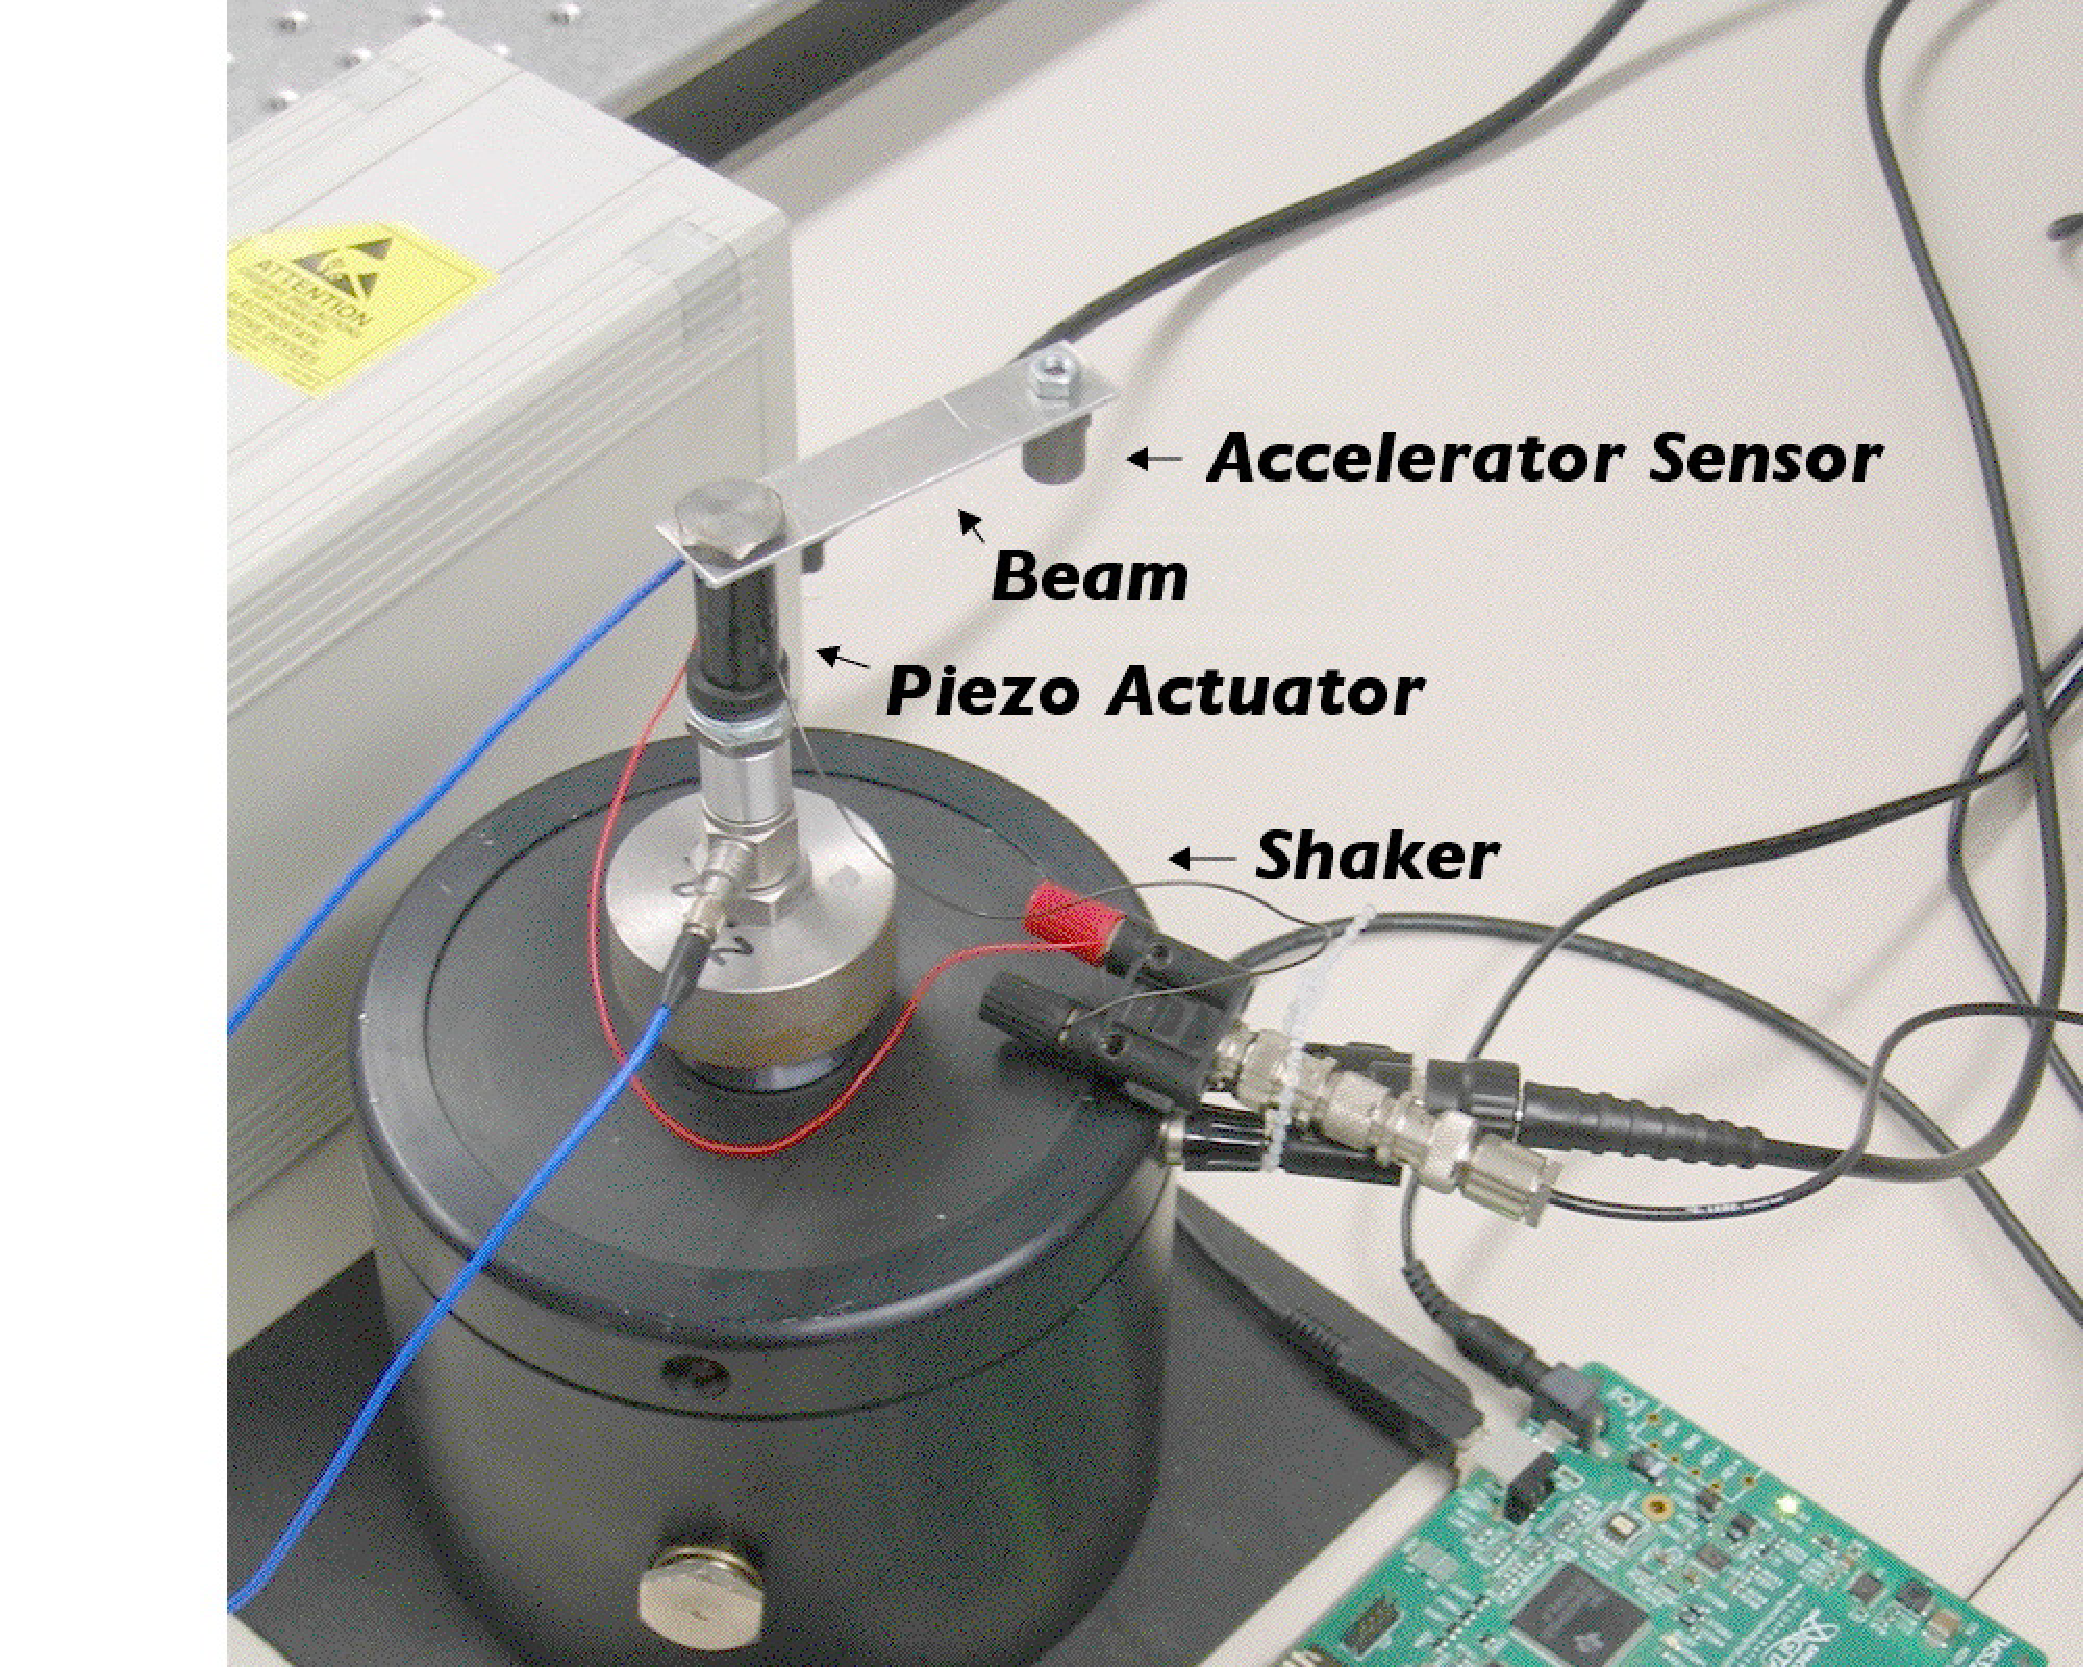
\includegraphics[scale=0.25]{../pdf/beam}
\caption{{\bf Piezo experiment}\label{beam}}
\label{default}
\end{center}
\end{figure}
The goal is to control  the actuator
using an adaptive FxLMS filter in order to dampen the resultant vibration of the beam. 

An adaptive FxLMS filter is determined by the following components:
\begin{center}
   \setlength{\unitlength}{0.9pt}   
   \begin{picture}(280,90)
   \put(-2,45){\footnotesize $x(n)$}
   \put(0,58){\vector(1,0){110}}
   \put(20,58){\vector(0,1){25}}
   \put(20,58){\circle*{3}}
   \put(20,58){\line(0,-1){45}}
   \put(20,13){\vector(1,0){20}}
   \put(40,0){\framebox(40,26){$\hat{S}(z)$}}
   \put(84,0){\footnotesize $x'(n)$}
   \put(80,13){\vector(1,0){30}}
   \put(110,0){\framebox(40,26){LMS}}
   \put(135,72){\vector(1,1){12}}
   \put(130,26){\line(0,1){20}}
   \put(150,13){\line(1,0){13}}
   \put(110,45){\framebox(40,26){$W(z)$}}
   \put(155,49){\footnotesize $y(n)$}
   \put(150,58){\vector(1,0){30}}
   \put(180,45){\framebox(40,26){$S(z)$}}
   \put(225,45){\footnotesize $y'(n)$}
   \put(220,58){\vector(1,0){26}}
   \put(250,58){\circle{8}}
   \put(250,85){\vector(0,-1){23}}
   \put(254,58){\vector(1,0){30}}
   \put(275,45){\footnotesize $e(n)$}
   \put(255,75){\footnotesize $d(n)$}
   \put(270,13){\line(0,1){45}}
   \put(270,13){\vector(-1,0){120}}
   \dashline[28]{5}(35,-5)(155,-5)
   \dashline[28]{5}(35,-5)(35,90)
   \dashline[28]{5}(35,90)(155,90)
   \dashline[28]{5}(155,-5)(155,90)
 \end{picture}
\end{center} 

\begin{itemize}
\item The actor-sensor system $S$ (secondary system) is comprised of the piezo actuator, the beam, and the accelerator sensor. Under the assumption that the filter $W(z)$ is 
linear and time invariant, the filter $W(z)$ and the secondary system may be switched. 
Replacing the secondary system by its model $\hat{S}$ results in the Figure above. 
The dashed line then include the FxLMS filter algorithm.

\item The adaptive FIR filter $w(z)$ specified
 by the difference equation $$y(n) = \sum_{i=0}^N w_{i} \cdot x(n-i)$$,

\item the stochastic LMS algorithm by the equation
$$w_{i}(n+1) = w_{i}(n) + \mu \cdot x(n-i) \cdot e(n)$$
where $e(n) = d(n) - y(n)$  is the error with $d(n)$ being the sensor signal.
\end{itemize}

This algorithm is active in state \pp{controlling} of the subsequent
program (with names being more meaningful). 
%
\codeinput{fxlms}
%
\begin{figure}[htbp]
\begin{center}
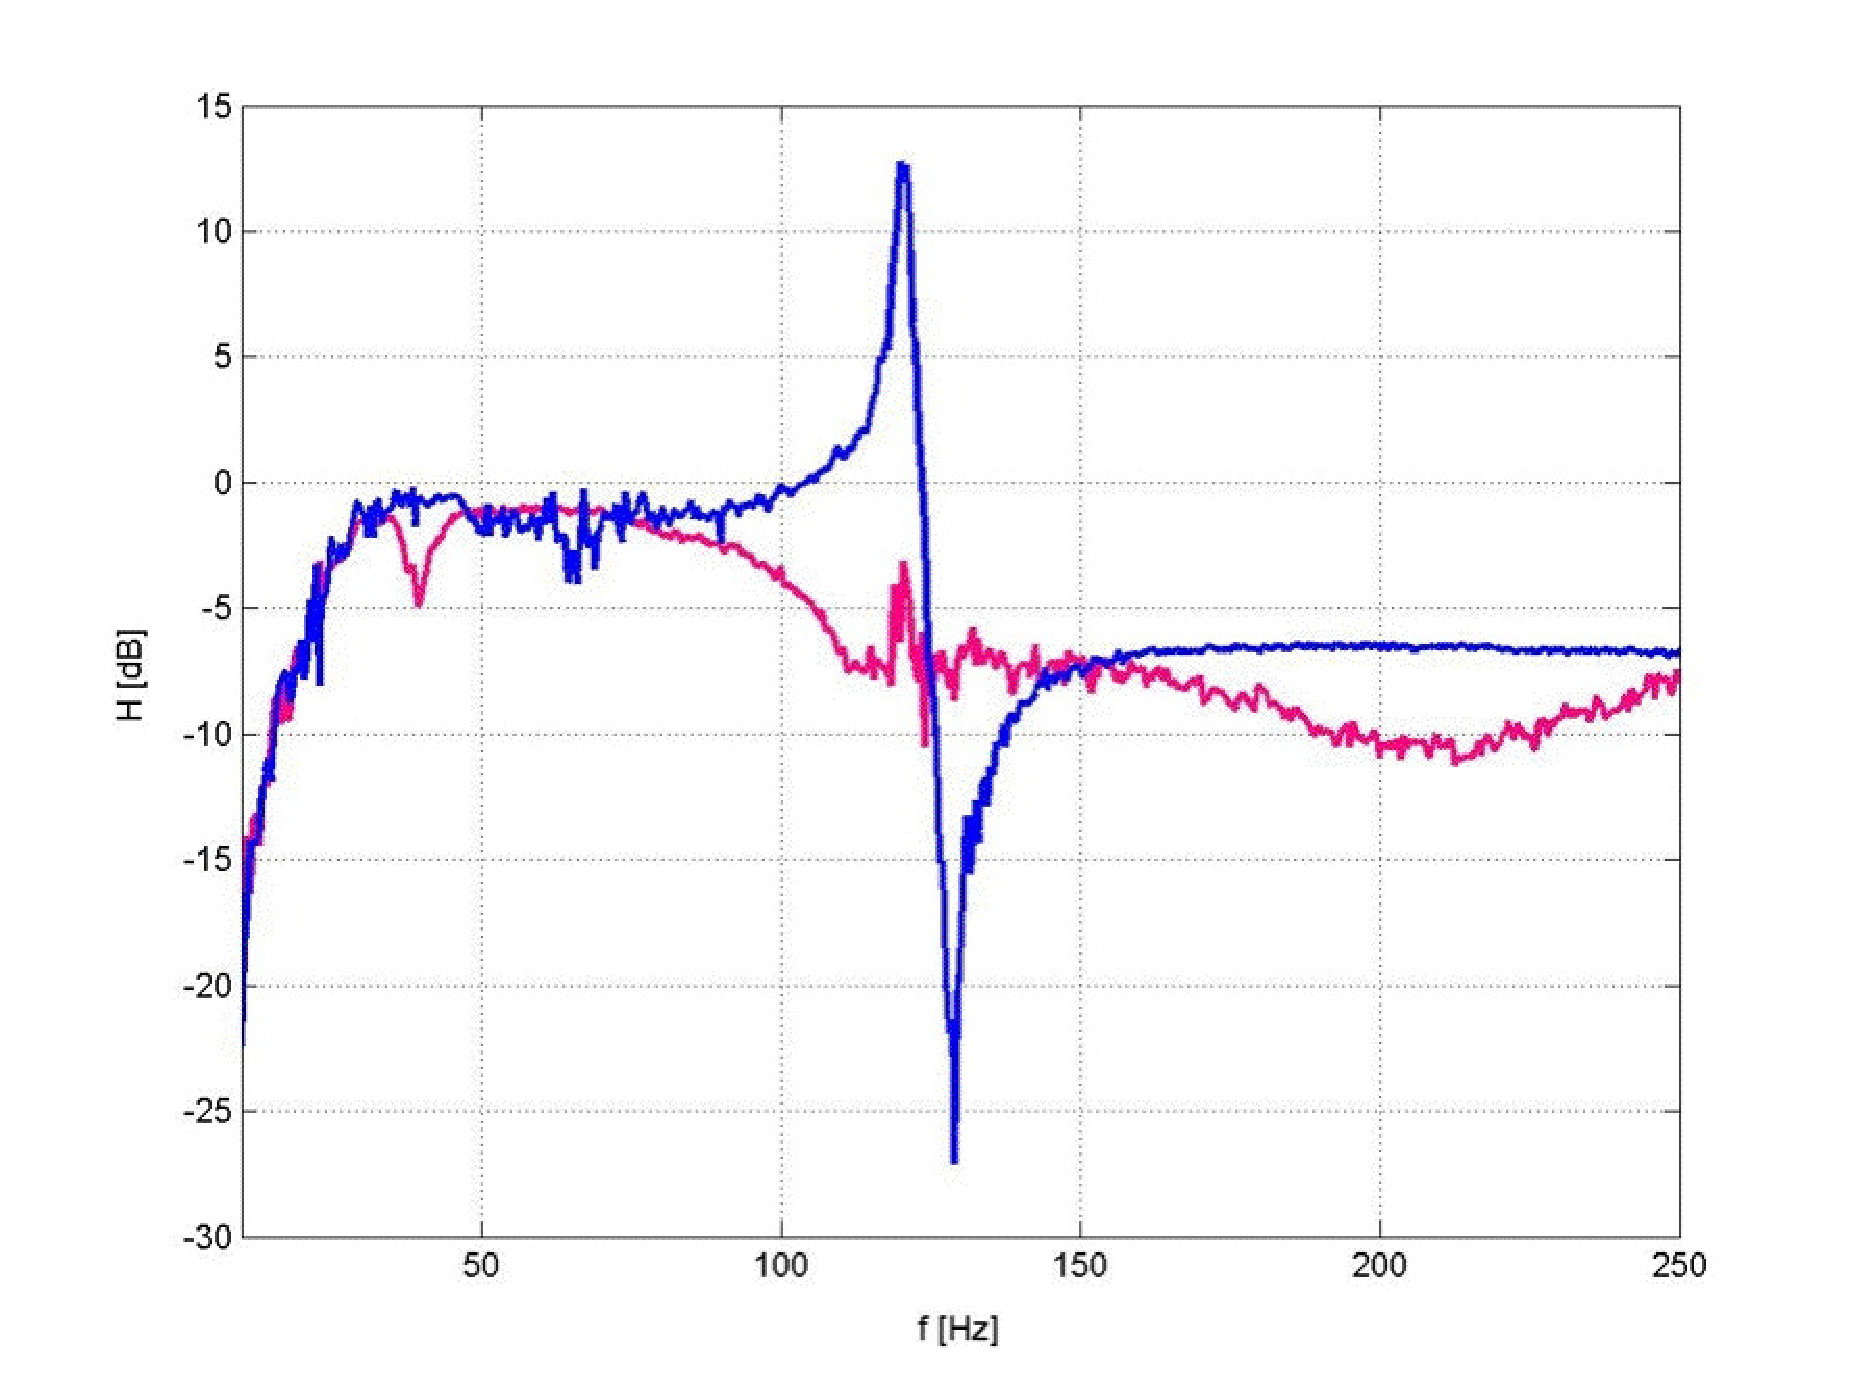
\includegraphics[scale=0.25]{../pdf/dampening}
\caption{{\bf Piezo experiment}\label{dampening}}
\end{center}
\end{figure}

There are two other states:
\begin{itemize}
  \item In state \emph{identify} system identification of the secondary
       system takes place, and

  \item in state \emph{shaker\_only} only the shaker is excited by the 
    native method \pp{noise-gen} which generates white noise. This state is meant
    provide a reference with regard controlled state in which the vibration is
    actively dampened by the piezo actuatuator. 
\end{itemize}
The results can be seen in Figure \ref{dampening}. The blue line specifies the undampened, the red line the dampened behaviour.

The program runs on a DSP evaluation board by Texas Instrument to be seen in Figure 
\ref{beam}. The board provides
a Codec and several Dip switches and Led's that are encapsulated in respective
input and output classes. The program is built and uploaded from the code as given.

\section{Representing State Models}

\paragraph{Dynamic systems a state model.} A \emph{state model} is a system of first-order coupled differential equations of the form
\begin{eqnarray*}
x'_{1} & = & f_{1}(t,x_{1},\ldots,x_{n},u_{1},\ldots,u_{p})\\
x'_{2} & = & f_{2}(t,x_{1},\ldots,x_{n},u_{1},\ldots,u_{p})\\
\vdots      &   & \vdots \\
x'_{n} & = & f_{n}(t,x_{1},\ldots,x_{n},u_{1},\ldots,u_{p})
\end{eqnarray*}
where $x'_{i}$ denotes the derivative of $x_{i}$ with regard to the time variable $t$, and $u_{1},\ldots,u_{p}$ are specified input variables. The variables $\dot(x)_{1},\ldots,\dot(x)_{n}$ are calle \emph{state variables}.


Linear time-invariant systems can easily be reformulated to a state model. Consider for instance the equations
\begin{eqnarray*}
L\frac{di(t)}{dt} +  Ri(t) + v_{c}(t)& = & v_{i}(t)
\end{eqnarray*}
and
\begin{eqnarray*}
v_{c}(t)& = & \frac{1}{C}\int_{-\infty}^td\tau
\end{eqnarray*}
describing an \textit{RLC}-circuit. Using the state variables $x_{1}(t) = i(t)$
 and $x_{2}(t) = v_{c}(t)$ substitution plus a few algebraic laws, we obtain
  the corresponding state model:
\begin{eqnarray*}
x'_{1} & = & \frac{R}{L}x_{1} + \frac{1}{L}x_{2} + \frac{v_{i}}{L}\\
x'_{2} & = & \frac{1}{C}x_{1}
\end{eqnarray*}

State models are quite a convenient representation for the numerical solution
of a system of differential equations on a computer. The method appropriate
for our purposes is the (forward) Euler method. Let 
\begin{eqnarray*}
\mathbf{x}'(t) & = & f(t,\mathbf{x},\mathbf{u})
\end{eqnarray*}
be a state mode (where $\mathbf{x}$ and $\mathbf{u}$ are vectorts). We replace the derivative by the difference approximation 
\begin{eqnarray*}
\mathbf{x}'(t) & \equiv & \frac{\mathbf{x}(t + dt)-\mathbf{x}(t)}{dt}
\end{eqnarray*}
which yields the formula
\begin{eqnarray*}
\mathbf{x}(t + dt) & \equiv & \mathbf{x}(t) + f(t,\mathbf{x},\mathbf{u})dt
\end{eqnarray*}
We can compute the estimates using the scheme
\begin{eqnarray*}
\mathbf{x}_{n+1} & \equiv & \mathbf{x}_{n} + f(t_{n},\mathbf{x}_{n},\mathbf{u}_{n})dt
\end{eqnarray*}
which naturally tranlates to \se. This is the \emph{(forward) Euler} method.

Similarly the \emph{backward Euler} method using
\begin{eqnarray*}
\mathbf{x}'(t) & \equiv & \frac{\mathbf{x}(t)-\mathbf{x}(t - dt)}{dt}
\end{eqnarray*}
for approximation can be used.

\paragraph{State models in \se.} We adopt the notation in that we allow ``primed'' signals in flow equations, e.g.
\BEP
  x1' := R/L * x1 + 1/L * x2 + vi/L\\
  x2' := 1/C * x1
\EEP
These equations will be a convenient shorthand for
\BEP
  x1 := pre(x1) + (R/L * x1 + 1/L * x2 + vi/L) * dt;\\
  x2 := pre(x2) + (1/C * x1) * dt;
\EEP
Note that this corresponds to backwards Euler. This is the more flexible
approach since we use the same scheme for
\BEP
  x1' := R/L * x1 + 1/L * pre(x2) + pre(vi)/L\\
  x2' := 1/C * x1
\EEP
to obtain forward Euler.

\paragraph{The bouncing ball example reconsidered.} We remember that the behaviour of a bouncing ball can graphically specified by the hybrid system
\begin{center}
	{\tt\small
       \thinlines
       \setlength{\unitlength}{0.9pt}
       \begin{picture}(140,100)
           \put(5,70){$x_{1} \leq 0$}
           \put(90,70){$x_{2} := -cx_{2}$}
           \put(65,76){\circle{50}}
           \put(79,59){\thicklines\vector(-2,-1){7}}
          \put(30,0){\Ovalbox{\begin{Beqnarray*}
                                      \\\ \dot{x_{1}} & = & x_{2}\
                                      \\\dot{x_{2}} & = & -g\\
                                 \end{Beqnarray*}}}       
       \end{picture}
     }
\end{center}
Hence one is tempted to translate this to
%
\codeinput{bouncing-ball-state-model-1}
%
However, this is not quite what we want since, according to the above,
the state equations translate to
\BEP
  x1 := pre(x1) + x2 * dt;\\
  x2 := pre(x2) + (-c * pre(x2) -> -g * dt;
\EEP
But the equations should be (cf. \ref{hybrid-system})
\BEP
  x1 := pre(x1) + pre(x2)* dt;\\
  x2 := (-c * pre(x2) -> x2) + -g * dt;  $(*)$
\EEP

For convenience, we add some notation which achieves just what is wanted
%
\codeinput{bouncing-ball-state-model-2}
%
Here the \pp{=>} indicates that the switch of in the previous value of the
signal. The corresponding equation $(*)$ is generated by preprocessing from
\pp{x2' := -c2 * x2 => -g}.




%Control engineers use \emph{signal flow graphs} for modelling processes.
%For instance,
%\begin{center}
%    {\footnotesize \setlength{\unitlength}{0.6pt}
%      \begin{picture}(190,120)
%	\thinlines \put(95,15){\circle*{10}} \put(140,15){\vector( -1,
%	0){40}} \put(145,15){\circle*{10}} \put(95,15){\vector( 0,
%	1){40}} \put(145,60){\vector( 0, -1){40}} \put(0,60){\vector(
%	1, 0){40}} \put(45,60){\circle*{10}} \put(50,60){\vector( 1,
%	0){40}} \put(95,60){\circle*{10}} \put(100,60){\vector( 1,
%	0){40}} \put(145,60){\circle*{10}} \put(150,60){\vector( 1,
%	0){40}} \put(45,105){\circle*{10}} \put(45,60){\vector( 0,
%	1){40}} \put(95,105){\circle*{10}} \put(50,105){\vector( 1,
%	0){40}} \put(95,105){\vector( 0, -1){40}}
%	\put(22,75){\makebox(0,0)[lb]{$z^{-1}$}}
%	\put(120,0){\makebox(0,0)[b]{$-b_1$}}
%	\put(180,65){\makebox(0,0)[b]{$y$}}
%	\put(70,65){\makebox(0,0)[b]{$a_0$}}
%	\put(5,65){\makebox(0,0)[b]{$x$}}
%	\put(70,110){\makebox(0,0)[b]{$a_1$}}
%	\put(172,32){\makebox(0,0)[rb]{$z^{-1}$}}
%      \end{picture}}
%\end{center}
%presents a recursive filter of first degree.  The values of ingoing
%arcs are added up, and the result is dispatched to the outgoing arcs.
%The labels are coefficients, $z^{-1}$ is time shifting operator for
%delaying by one unit of time.

%The signal flow graph is a presentation of the difference equation
%% 
%$$y(n) = a_0 * x(n) + a_1 * x(n-1) - b_1 * y(n-1),$$
%% 
%with the time index $n \in I\!\!N_o$ and the initial condition $y_0 = 
%a_{0} * x(t_{0})$.

%

%
%\section{More Examples}
%

%\subsection{A Lift Controller}

%A lift moves and stops while reacting to requests caused by pressing buttons. There are three kinds of buttons, \emph{lift} buttons, and \emph{up} and \emph{down} buttons. The 
%lift buttons are in the lift.\footnote{The example solution is 
%a transcription of a Lustre program designed by Leslek Holenderski~\cite{holenderski}.}

%\subsection{The Production Cell}

%Leszeks example







